\chapter{Parameter estimation and model comparison}

For the proposed models, exploration of the uncertainties in the parameter estimations is our main task in this chapter, which involved the application of ABC SMC and several experiments. After that, the parameter inference framework was also used for model selection.

The build and test of the code were under \verb|Python| environment with \verb|pyABC|\cite{ref:pyabc}. Some other code, e.g. shell scripts and \verb|R| code were also used to perform the experiments and result analysis. Software and system environment used in our implementation can be found in Appendix A. The build and test were performed on local computers and HPC facilities available within EPCC.

\section{Code and implementations}

%  [ABC implementations details, e.g. distance, population, ODE related functions]

%  [how the code is developed and built]

According to our preliminary studies, a ABC SMC framework implemented using \verb|pyABC| in \verb|Python| was adopted in this project. \verb|pyABC| is a popular SMC software packages\cite{ref:pyabc} which has been used form many ABC SMC inference applications\cite{population}. \verb|pyABC| provides an open-source framework for likelihood-free inference, which is a \verb|NumPy| implementation of ABC SMC algorithm and a useful tool-box for our own inference and analysis tasks. Besides, it supports multi-core execution implemented using \verb|multiprocessing| built-in package, and it made our further studies in the scaling-up performance possible.

%  which is of our interests and suitable for the followed performance experiments.

The inference framework code for the project was developed and tested in local environment (macOS 10.15.6, see Table \ref{table:local_macine}) at first using a small input, then the functional version was deployed on compute node of ARCHER and Cirrus for parameter inference experiments and model selection tasks. The scaling-up experiment was performed on Cirrus. The profiling and its analysis were performed on local machine. Some necessary development and debug were performed on the remote machines to ensure that experiments run correctly on compute node.

The ODE model-related code and utilities were firstly developed to enable reusable functions, variables and data calls. It included the code for the ODE equations, ODE solver, data structures and data format transform functions, etc. By doing this in separate code files, we could change implementation options and activate ABC SMC easily in another `trigger' file, without creating definition and duplicated code for the models, observed data and parameter priors.

Some missing features were found when using \verb|pyABC|, therefore some modifications were made to the source code of \verb|pyABC|.

For example, the laboratorial measured data were not considered `complete' or `tidy' for modeling and analysis purpose: the available time points for cells and cytokines were different, e.g. cell number was not measured at 0.25 hpl and cytokines' expression was not measured at time point 120 hpl. These missing values were treated as `ignored' when calculating the distance between observed data and simulated data, and represented by \verb|NaN|s. However, in some distance calculations \verb|NaN| was not acceptable; to cope with this, built-in distance function was modified. Other modified code include some visualisation and result representation enhancements

Analysis of the program output was also wrapped up into functions which can be easily called after an ABC SMC run is finished, which includes multiple visualisations and summary statistic of the results. For different tasks there are also separated analysis code file. Other analysis tools used in the project include built-in database visualisation tool, R code and Microsoft Excel.

The project code was managed via \verb|git| version-control and available as a GitHub repository\footnote{\url{https://github.com/chaolinhan/MSc_Project}}; it also made the cross-hardware synchronisation of code versions convenient.

After several development iterations, code files for ABC SMC implementation now mainly had two types: code files for infer-back experiments (udsing synthetic data), and code files for parameter inference (using experimental data). Model selection can be easily done by adding more model to the implementation code file.


% \section{Parameter estimation}

% [implementation details and options/ settings that are affecting the ABC]





\section{Hyperparameters and implementation options experiments}

As the key focus of this project was on the parameter estimations of dynamical system, the ability of inference on the proposed models was firstly examined before actual inference using the experimental observed data.

In the first part, synthetic data is used with known true parameter values. The algorithm implementation is evaluated by the efficiency and goodness of resultant model under different implementation options and ABC SMC hyperparameters.

Then according to findings in the first part, several options with good performance are tried in the inference using experimental observed data (Figure \ref{fig:obs_data}). To obtain a more accurate and general results, these experiments are repeated for 3 or more times.

    % [including the options that are tested/ tried/ not adopted]

    % [including experiments results and discussions]

    % [how do these options correspond to biological model and how to set them accordingly for proposed model]

    % [why use synthetic data]

The ABC SMC inference can have largely different performance when using different hyperparameters and implementation options. To firstly test the ability of inference and observe the results of different options, synthetic data with known true parameter values are used as target data. by doing this, we could directly compare the inferred parameters to the true value, and compare the simulated trajectories to the true trajectories and then observe the result to see whether the inference is successful and how well the model fit the data. Also, by setting the same final threshold value, the efficiency under different options can be compared and help us to choose proper options when applying ABC SMC on the observed data. The true value of parameters that were used to generate synthetic data is listed in Table \ref{table:known_values}. 

The true values were obtained by fitting model 1 onto the experimental data (Figure \ref{fig:infer_back_data}) using least-square optimisation method. Available least-square fit tools in \verb|SciPy| were used. The fit algorithm was Trust Region Reflective\footnote{\url{https://docs.scipy.org/doc/scipy/reference/generated/scipy.optimize.least_squares.html}}. Target data was then generated using these parameter values via ODE integrate solver\footnote{\url{https://docs.scipy.org/doc/scipy/reference/generated/scipy.integrate.odeint.html}}.


\begin{figure}[ht]
    \begin{center}
        \resizebox{1.0\hsize}{!}{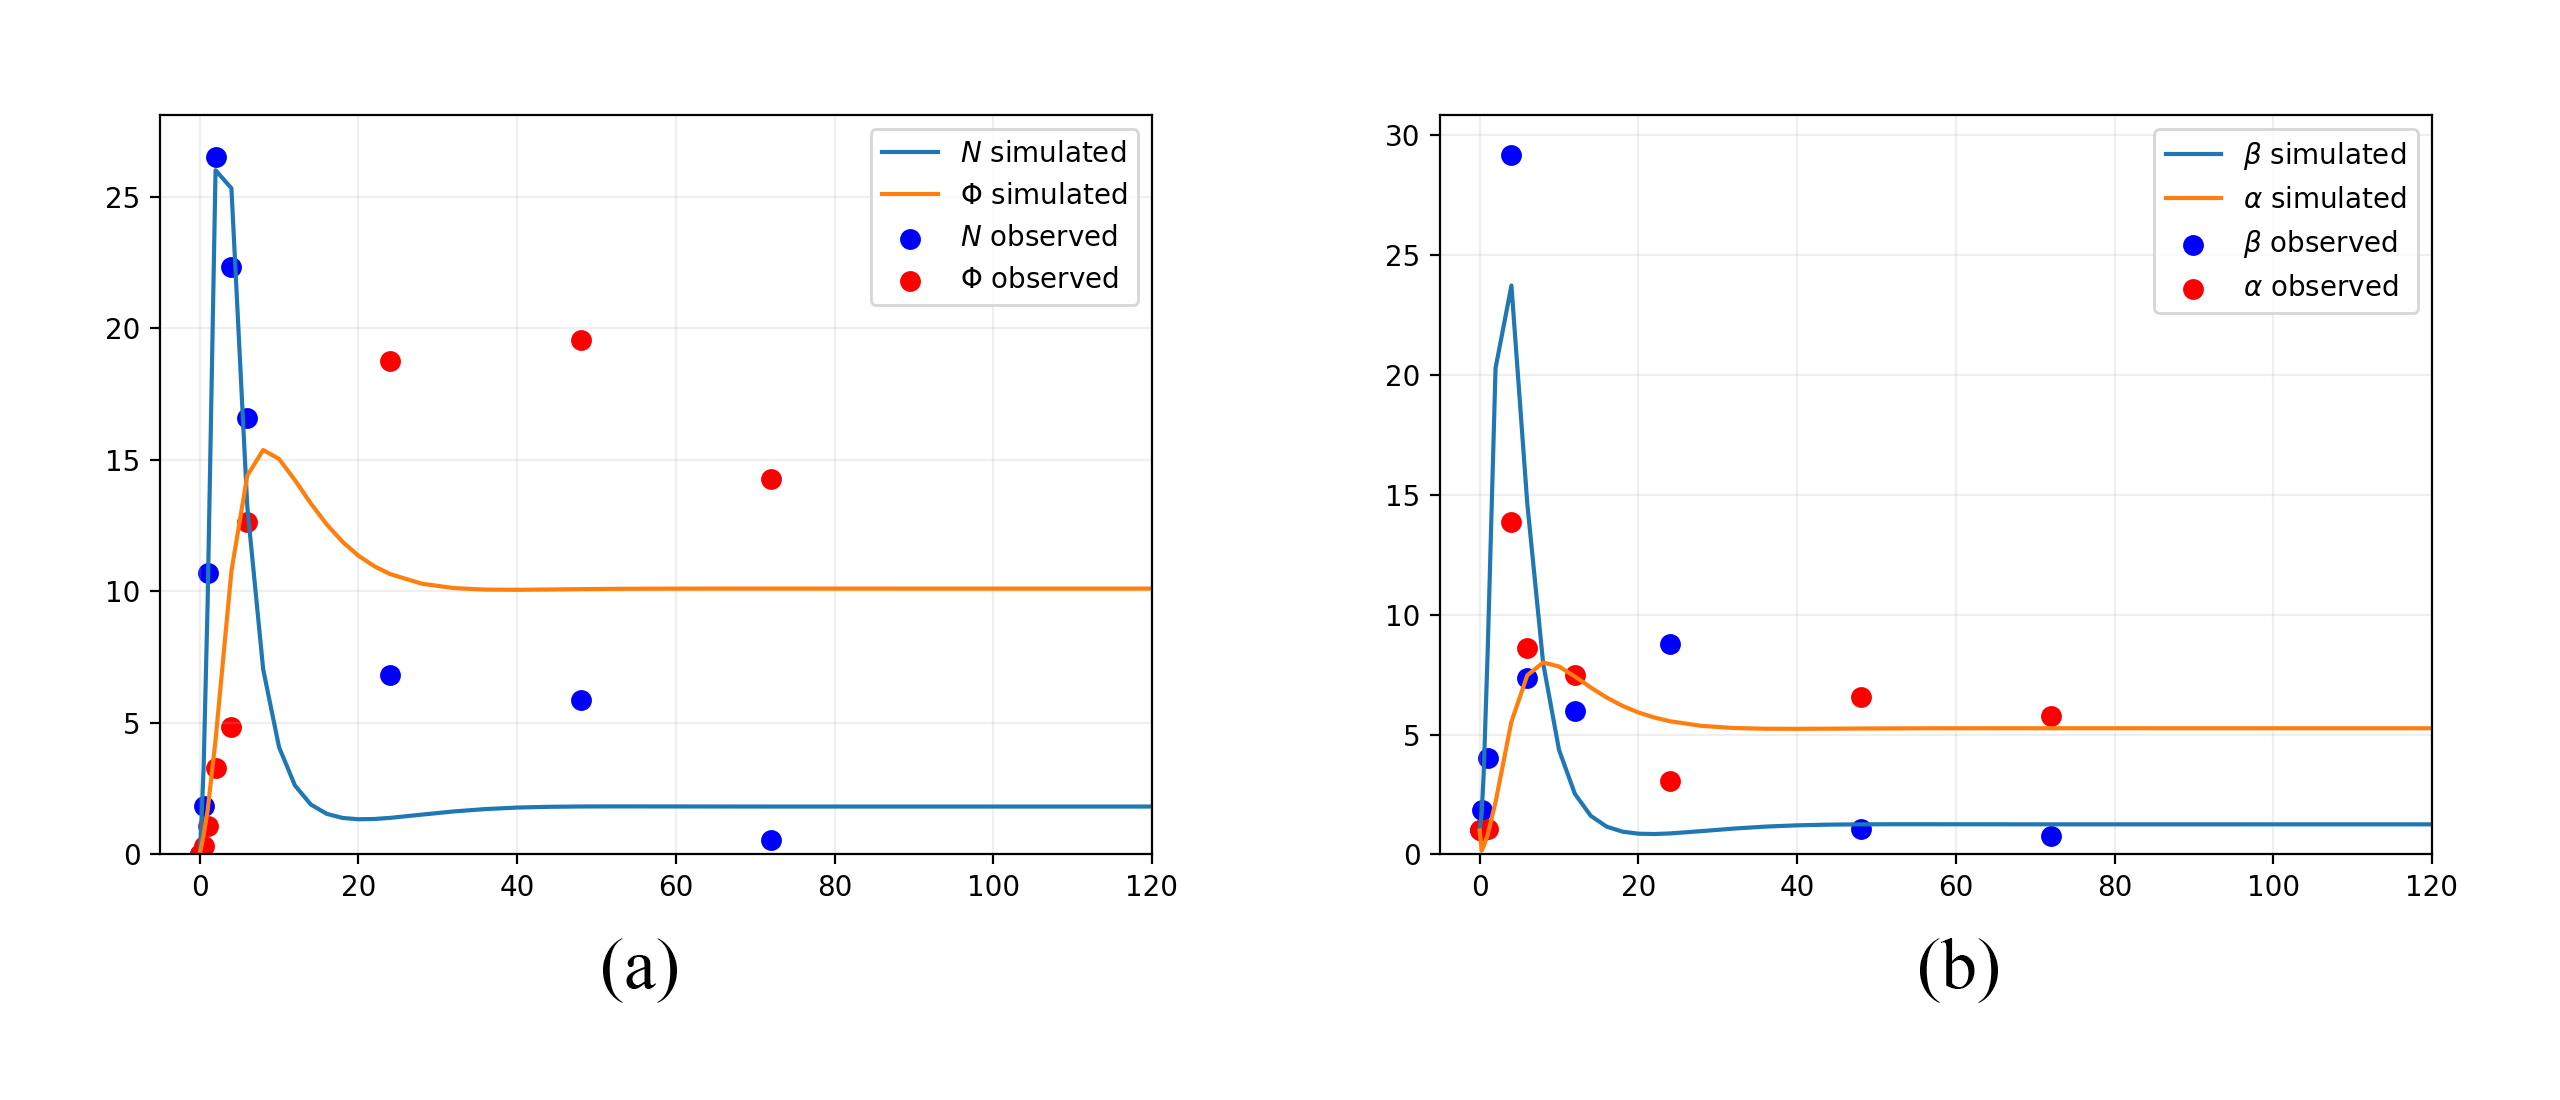
\includegraphics{fig/LS.png}}
    \end{center}

    \caption[Synthetic data generated with known parameter values]%
    {Synthetic data generated with known parameter values (line plot), compared to experimental data (scatter plot). Known parameter values are obtained from a least square fitting of the observed data}
    \label{fig:infer_back_data}

\end{figure}


Among them the following topics are studied using the synthetic data.

\subsection{Perturbation kernels}

Perturbation kernels work in the sampling process. In each generation $t$, samples are firstly taken from the previous population $\{\theta_{t-1}\}$ with weights $\{w_{t-1}\}$, then perturbed using the perturbation kernel $K(\theta|\theta^*)$. We keep sampling until $N$ particles are accepted, where $N$ is the pre-set population size. After that the new weights are calculated and normalised.

% \begin{figure}[t!]
%     \begin{center}
%         \resizebox{1.0\hsize}{!}{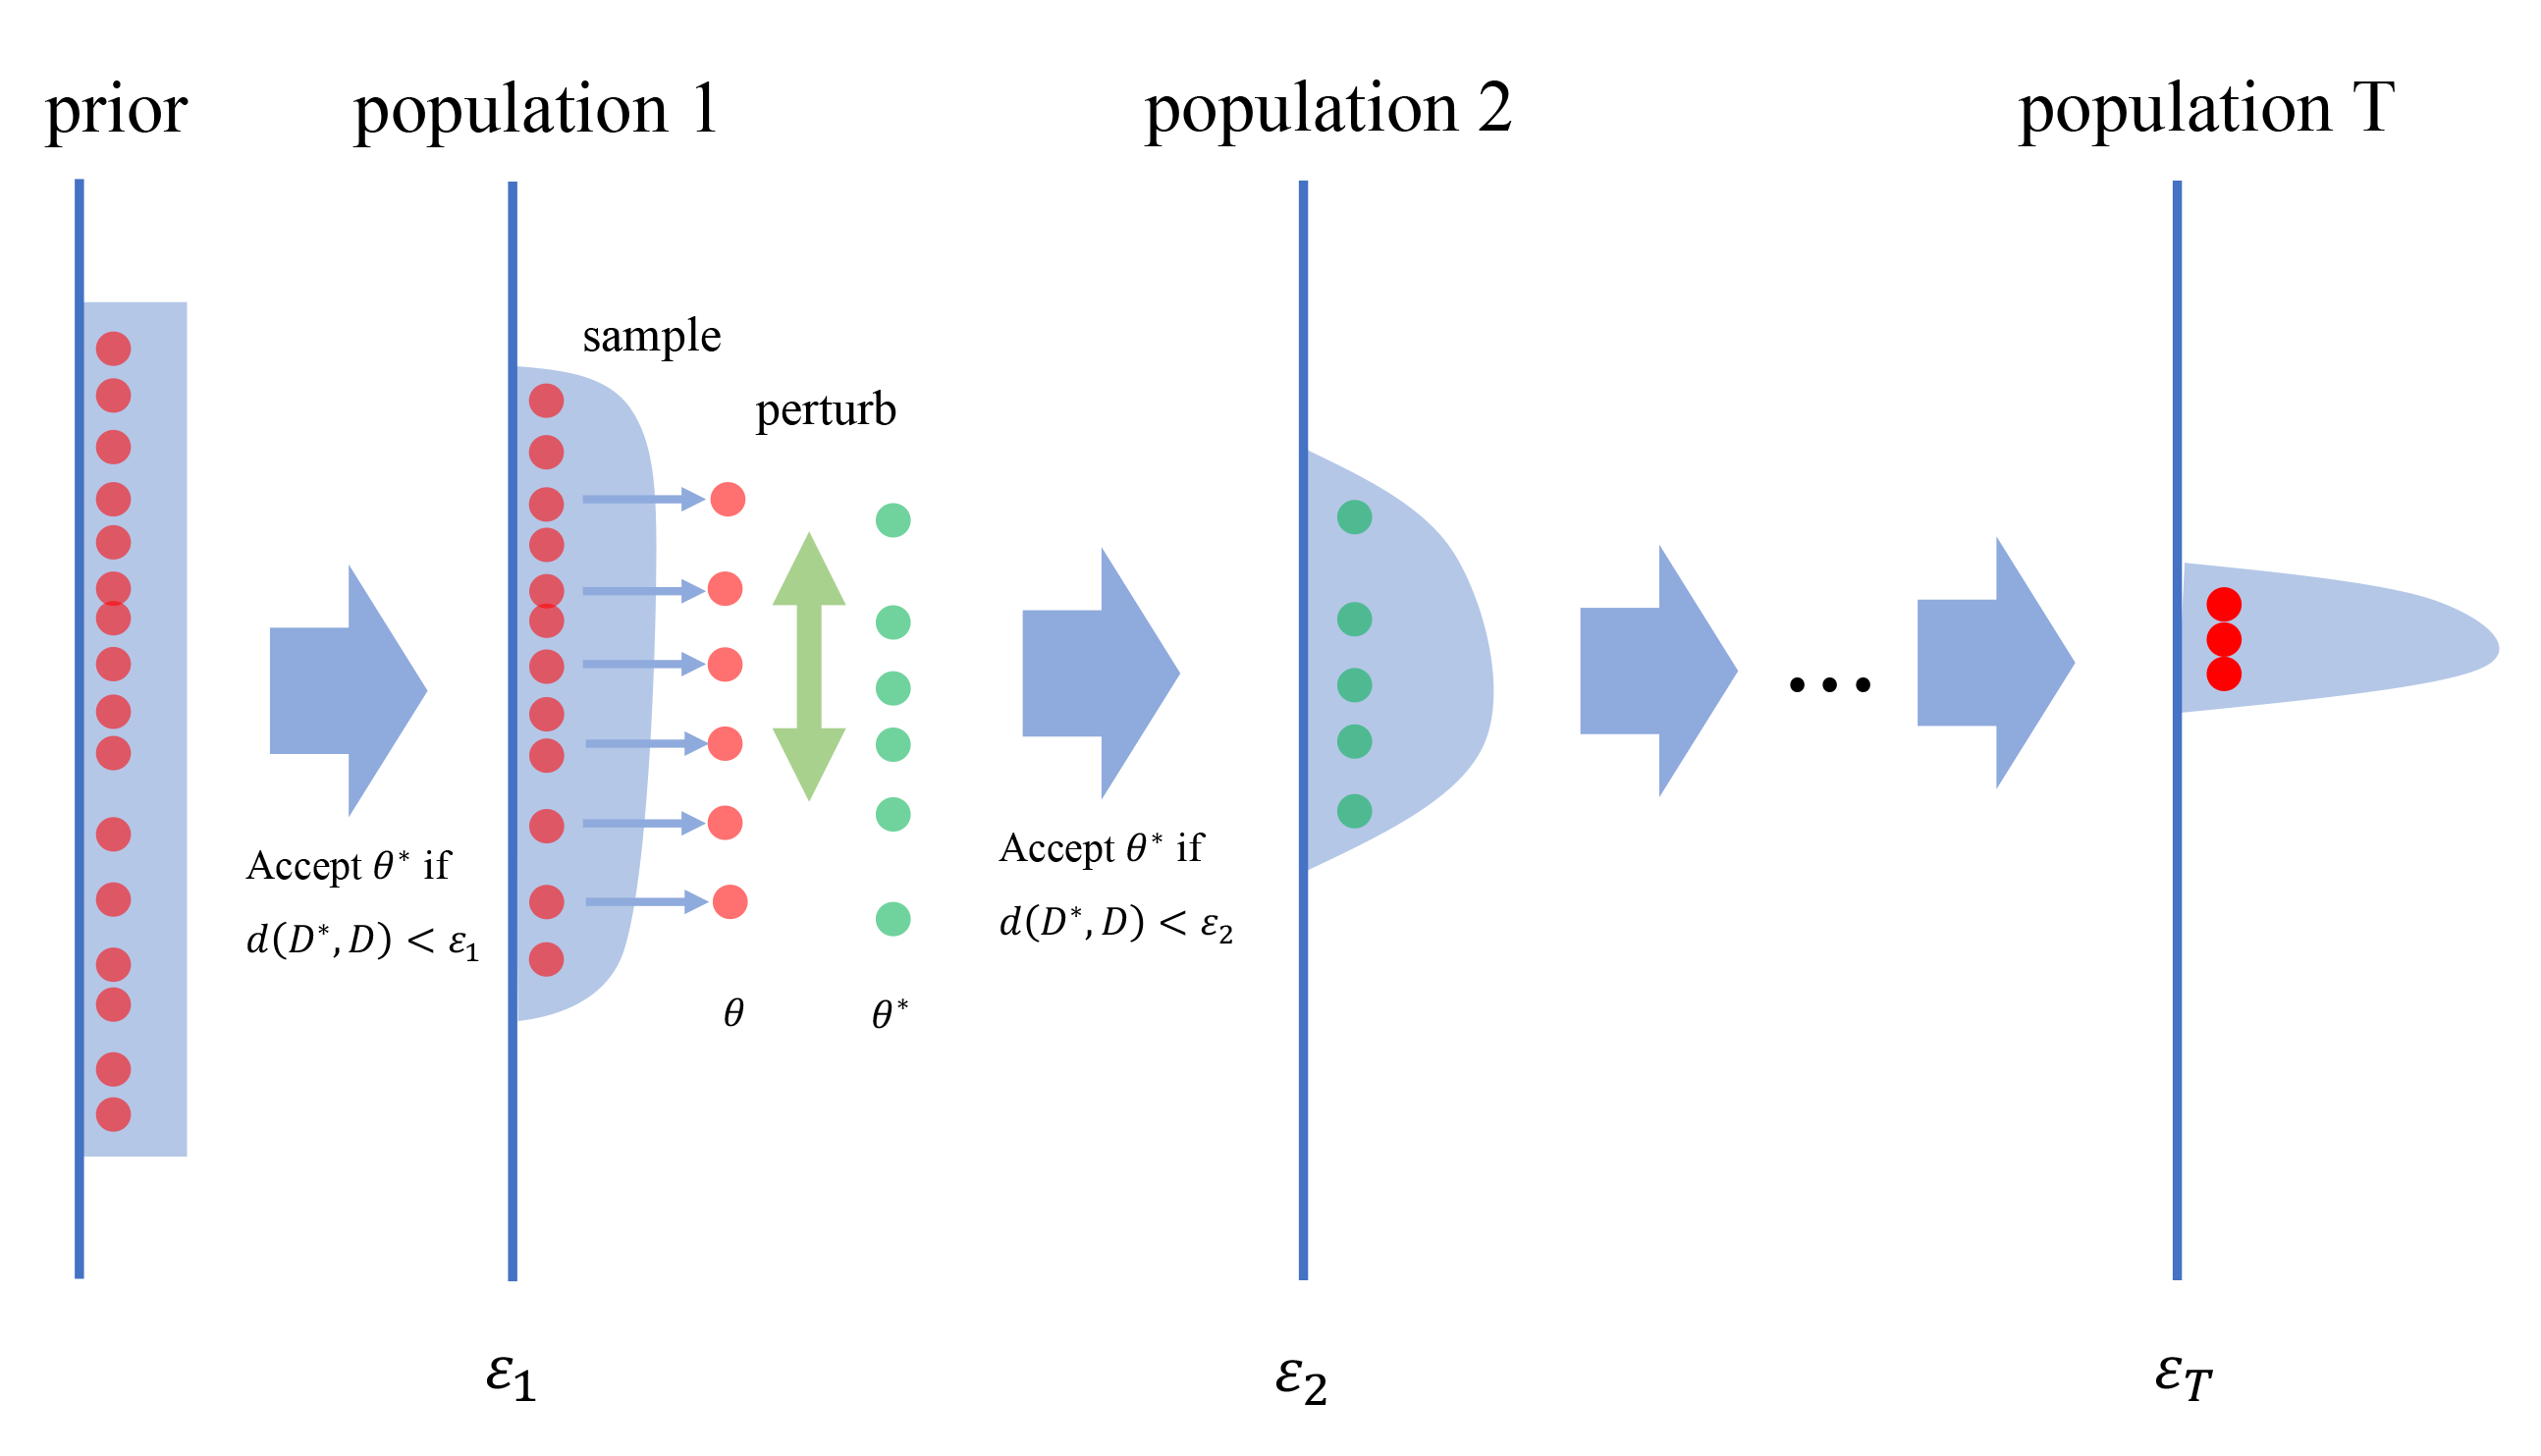
\includegraphics{fig/smc.png}}
%     \end{center}

%     \caption[ABC SMC sampling process]%
%     {ABC SMC sampling process. $\theta^*$ denotes a sample drawn from previous population, which is used to generate simulated data $D^*$. $d$ is a distance measurement, $d(D^*,D)$ represents the discrepancy between observed data and simulated data. for each population $t$, $\epsilon_t$ is a threshold criterion to determine whether to accept that drawn sample}
%     \label{fig:smc}

% \end{figure}

The perturbation kernel is called in the sampling of every particles and determines how the new perturbed particle is chosen, thus it is influential to both computation complexity and the resultant posterior distribution. Generally, a local perturbation kernel may face the risk of being stuck in local modes (e,g., local optimal), but it may need less computational operations, or could generate a population with a higher acceptance rate if the successive epsilon values are close; A kernel with wide variance, or spreading out in a large space could help in resolving the local optimal problem by a more thoroughly exploration of the parameter space, however it can be more computation-intensive and result in a lower acceptance rate. A desired optimal kernel should balance the trade-offs; their property and criteria is discussed in \cite{ref:kernel}.

There are several common choice of perturbation kernels. Among them multivariate normal kernel and local M-nearest neighbour model is preferred to be applied on our models. A covariance matrix $\Sigma_t$ of accepted particles is calculated form previous generation and used in multivariate normal kernel: $K(\theta|\theta_{t-1})\sim\mathcal{N}(\theta_{t-1}, \Sigma_t)$. It is illustrated to be more efficient than uniform kernel and component-wise normal kernel in relecting the true posterior structure \cite{ref:kernel}. It has been proved to perform well in several dynamic system models \cite{ref:abcsysbio, ref:compare, ref:disease} for the parameter estimation and model selection tasks. The $scaling\in(0,1]$ parameter in \verb|pyABC| will be multiplied to the covariance to produce a `narrower distributed' perturbation result.

Local M-NN kernel provided by \verb|pyABC| is also tried to provide a comparison. A local kernel density estimation (KDE) fit is used with M nearest neighbours considered.

The kernel experiments is designed to explore the efficiency of SMC on our dynamical systems. Given the same fixed threshold schedule, kernels that need less total samples and have higher acceptance rate would be our preference. The experiments compared multivariate normal kernel with local MNN kernels with different parameters, using synthetic data to infer back the parameters. The acceptance rate among each time point and total required samples are compared after the experiment to give suggestions on the kernel selection in the real data inference. As the threshold schedule is fixed, the final population should have similar discrepancy to the target data thus here the goodness of fit i.e. recover of target data trends/features and errors of the inferred parameters compared to true values is not discussed.

\subsubsection{Kernel experiment results}

To compare kernels, a fixed schedule schedule is used with minimal epsilon i.e. $\epsilon_t$ set to 10.0. From the total required samples graph Figure \ref{fig:kernel1}, the efficiency can be compared. Among the tested kernels, the local M-NN with M=50 has the best performance: it requires the least number of samples and
has higher acceptance rates among almost all generations. Local M-NN with M=750 is the slowest kernel.

For local M-NN kernels, generally a greater M will lead to lower acceptance rate and
more required particles in each generation. As shown in Figure \ref{fig:acceptance1}, local M-NN with M=750 is the lowest curve. Consequently, if greater M is test, then it will have even lower acceptance rates; the maximum M=2000 (whole population is considered) will have the lowest acceptance rates.

\begin{figure}
    \begin{center}
        \resizebox{1.0\hsize}{!}{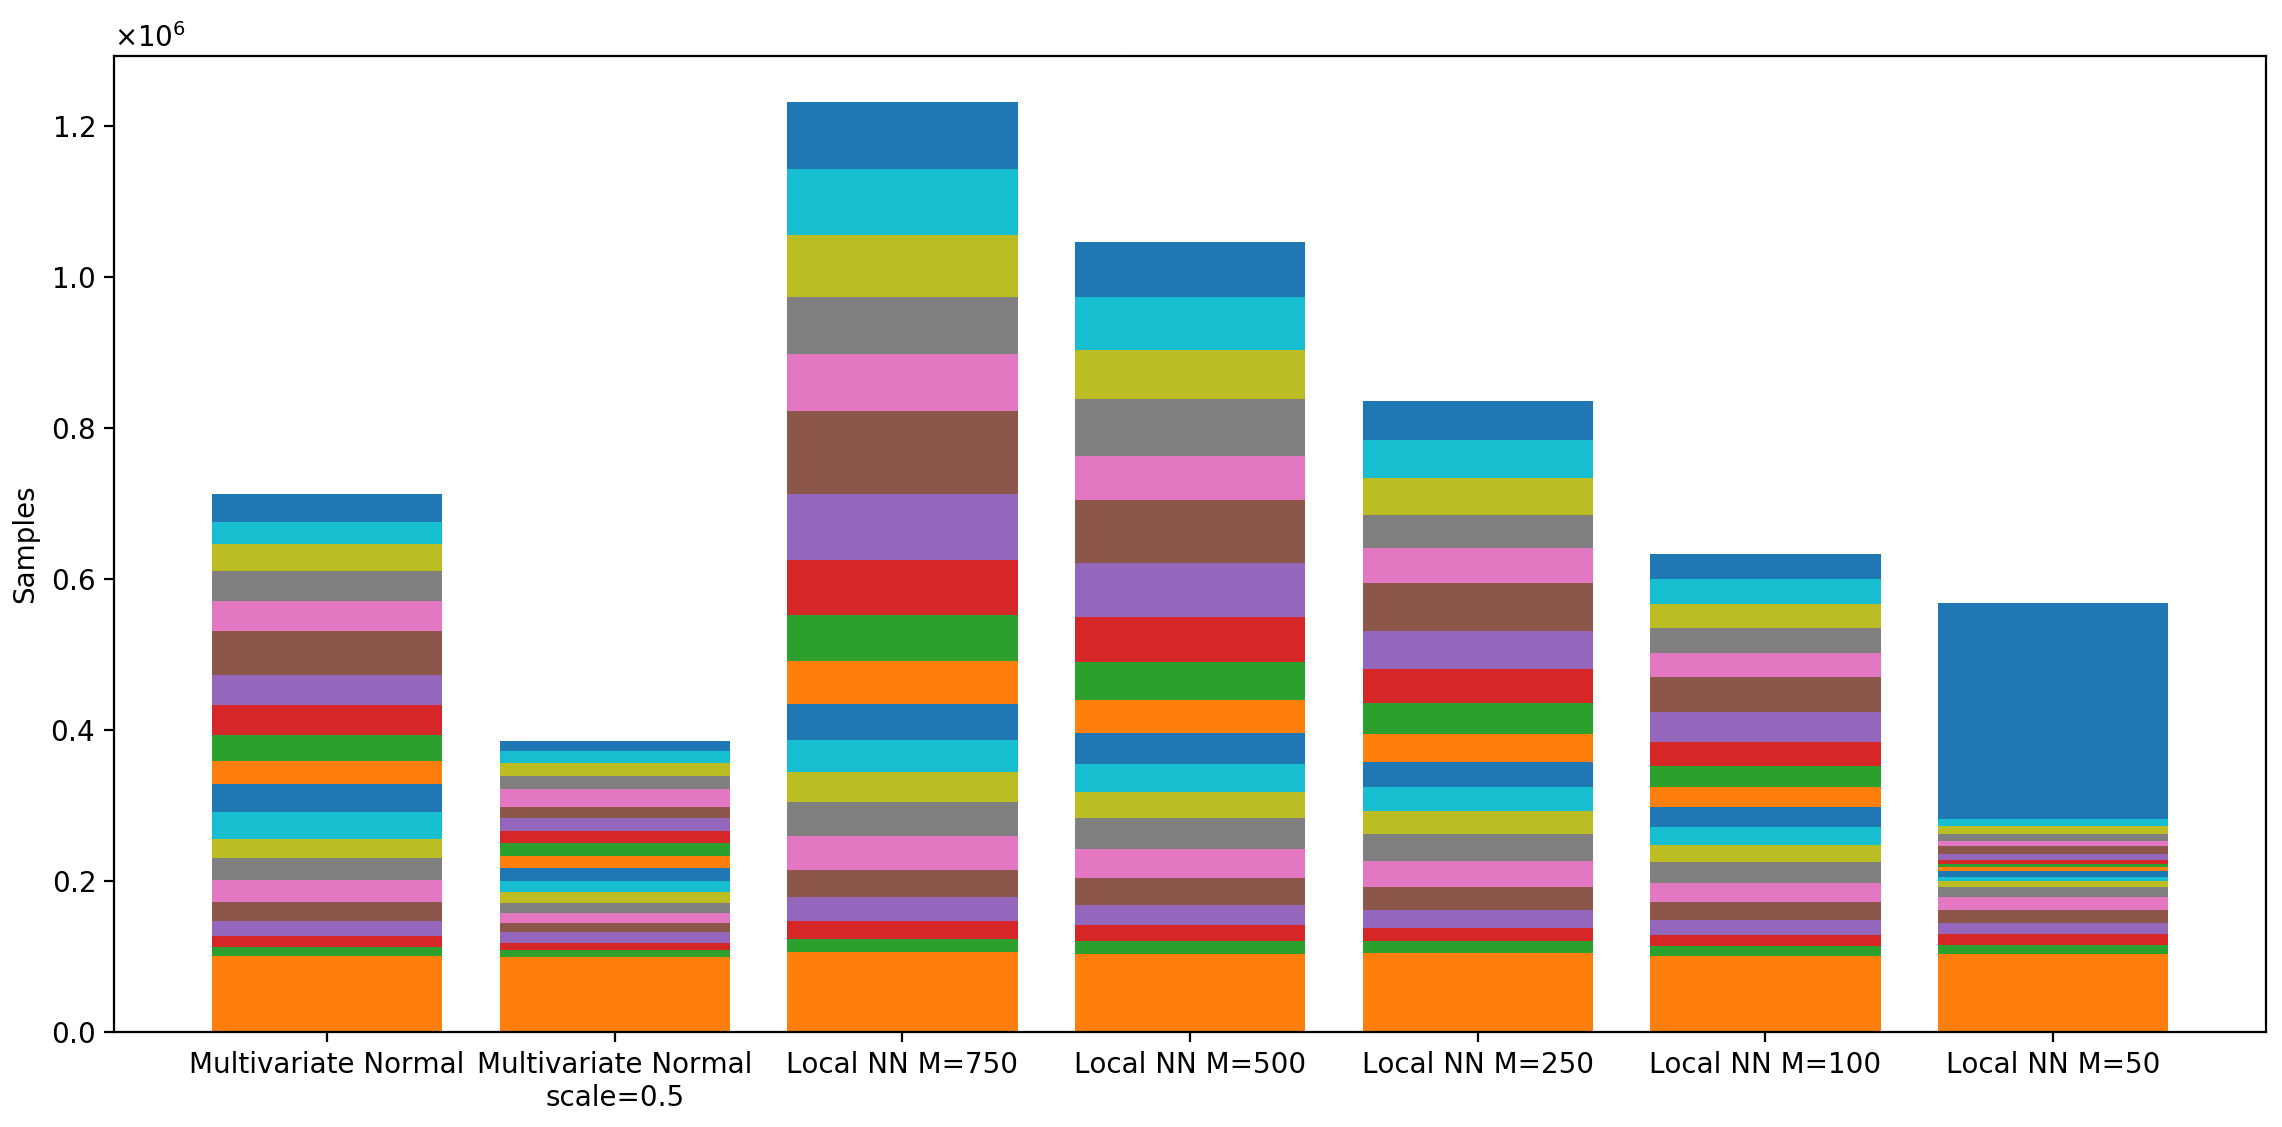
\includegraphics{fig/kernel1.png}}
    \end{center}

    \caption[Total required samples of different kernels]%
    {Total required samples of different kernels after 20 populations (2000 particles in each population). Different color represents different generations (bottom to top: population 1 to population 20)}
    \label{fig:kernel1}

    \vspace*{\floatsep}

    \begin{center}
        \resizebox{1.0\hsize}{!}{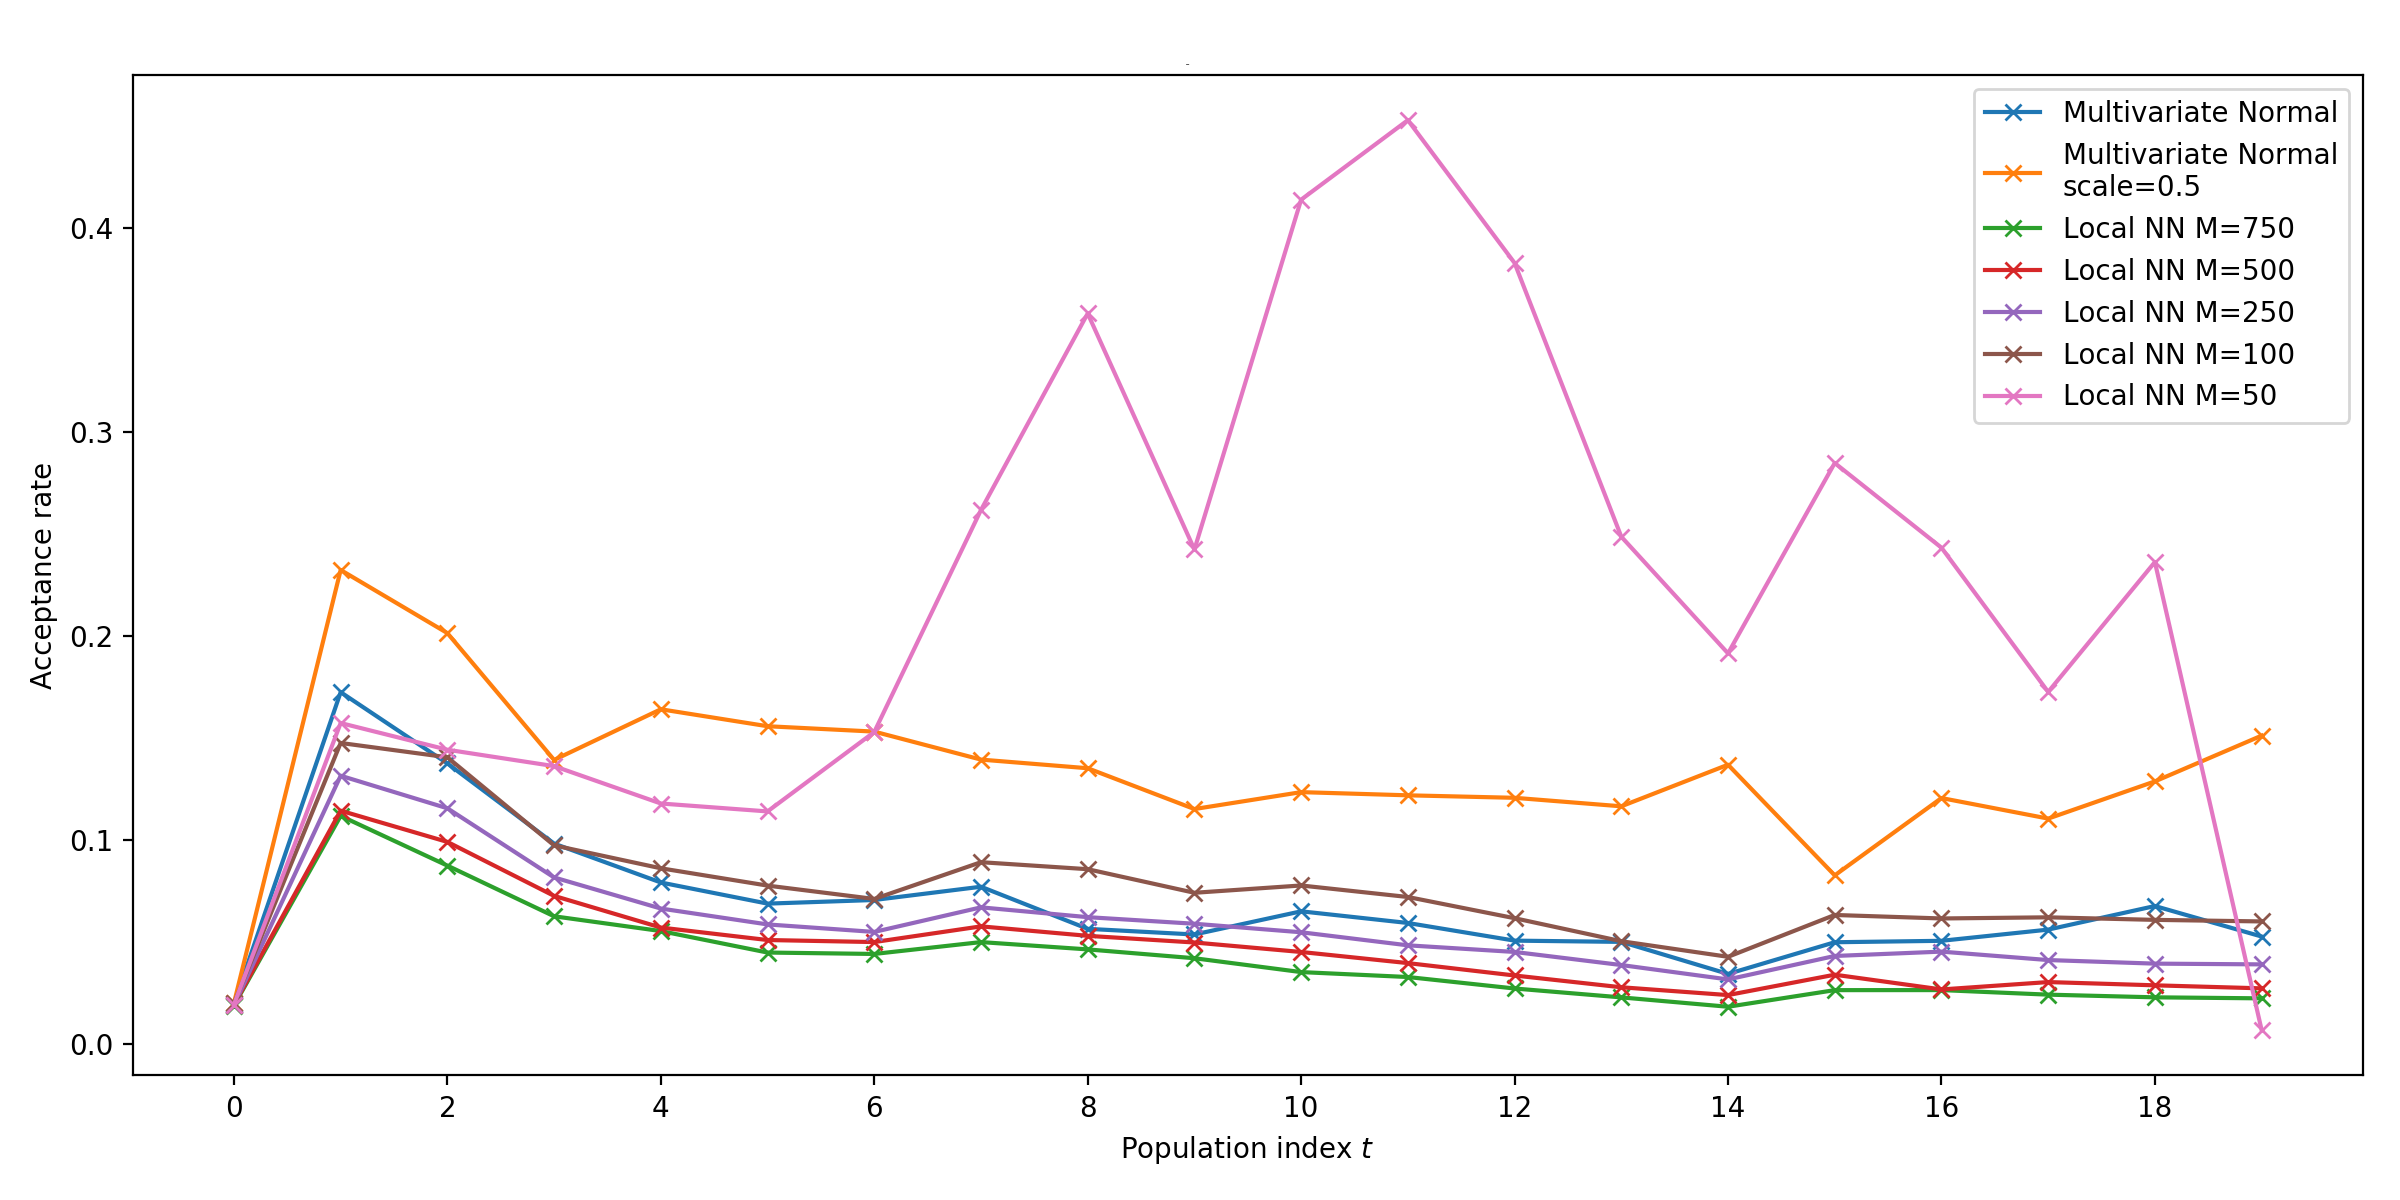
\includegraphics{fig/acceptance1.png}}
    \end{center}

    \caption[Acceptance rates of different kernels]%
    {Acceptance rates of different kernels in 20 populations. Each population has 2000 particles}
    \label{fig:acceptance1}

\end{figure}

Multivariate normal kernel has a performance between local M-NN M=250 and M=100. It proves that rather than a trivial normal kernel, multivariate normal kernels is more efficient facing the concentrations of joint distributions among multiple parameters \cite{ref:kernel}. `Scaling' option can narrower the distribution calculated from the last population, thus making the kernel more `local' by sampling under a smaller variance. Similar to small M in local M-NN, small `scaling' is also more efficient in our experiment of the model 1. Besides the fixed threshold schedule, a median threshold schedule with the same final threshold $\epsilon_{20}=10.0$ is also tested and similar results are observed (Figure \ref{fig:kernel2} and \ref{fig:acceptance2}, Appendix B2).

It seems that a more `local' kernel can give better performance by efficiently sampling around concentrations in parameters' distribution and approximate the posterior distribution. This holds in most cases under a given target final threshold value $\epsilon_t$, however may not produce the proper result want: a more local kernel, e.g. local M-NN with small M and multivariate normal with `scaling' is more likely to be stuck in local optimality, as the kernel is less likely to sample particles that are far from local concentrations, although these local optimal are still accepted under given threshold. In other words, using local kernels the epsilon may quickly converge to to local optimal; if a even smaller epsilon is desired, the local kernel can hardly generate enough particles to find another matched local modes. Also, the shapes of posterior distribution will affect the performance of local kernels \cite{ref:kernel}. One obvious example is presented in Figure \ref{fig:kernel1}, where local M-NN with M=50 suffered from a local optimal: the last generation takes much more samples to meet the required threshold.

\subsubsection{Conclusion} Local kernels can be fast bur unstable in some case; for a general parameter inference of our models, multivariate kernels are preferred, as a good fit is our prior target; some local kernels are also worth trying after the multivariate normal kernel, e.g. local M-NN with M$\leq 250$ (for population size of 2000, i.e. 12.5\% of the population) and multivariate normal with scaling. Also multivariate M-NN is worth trying, although it is not built in \verb|pyABC| and requires additional implementations.


% \begin{figure}
%     \begin{center}
%     \resizebox{1.0\hsize}{!}{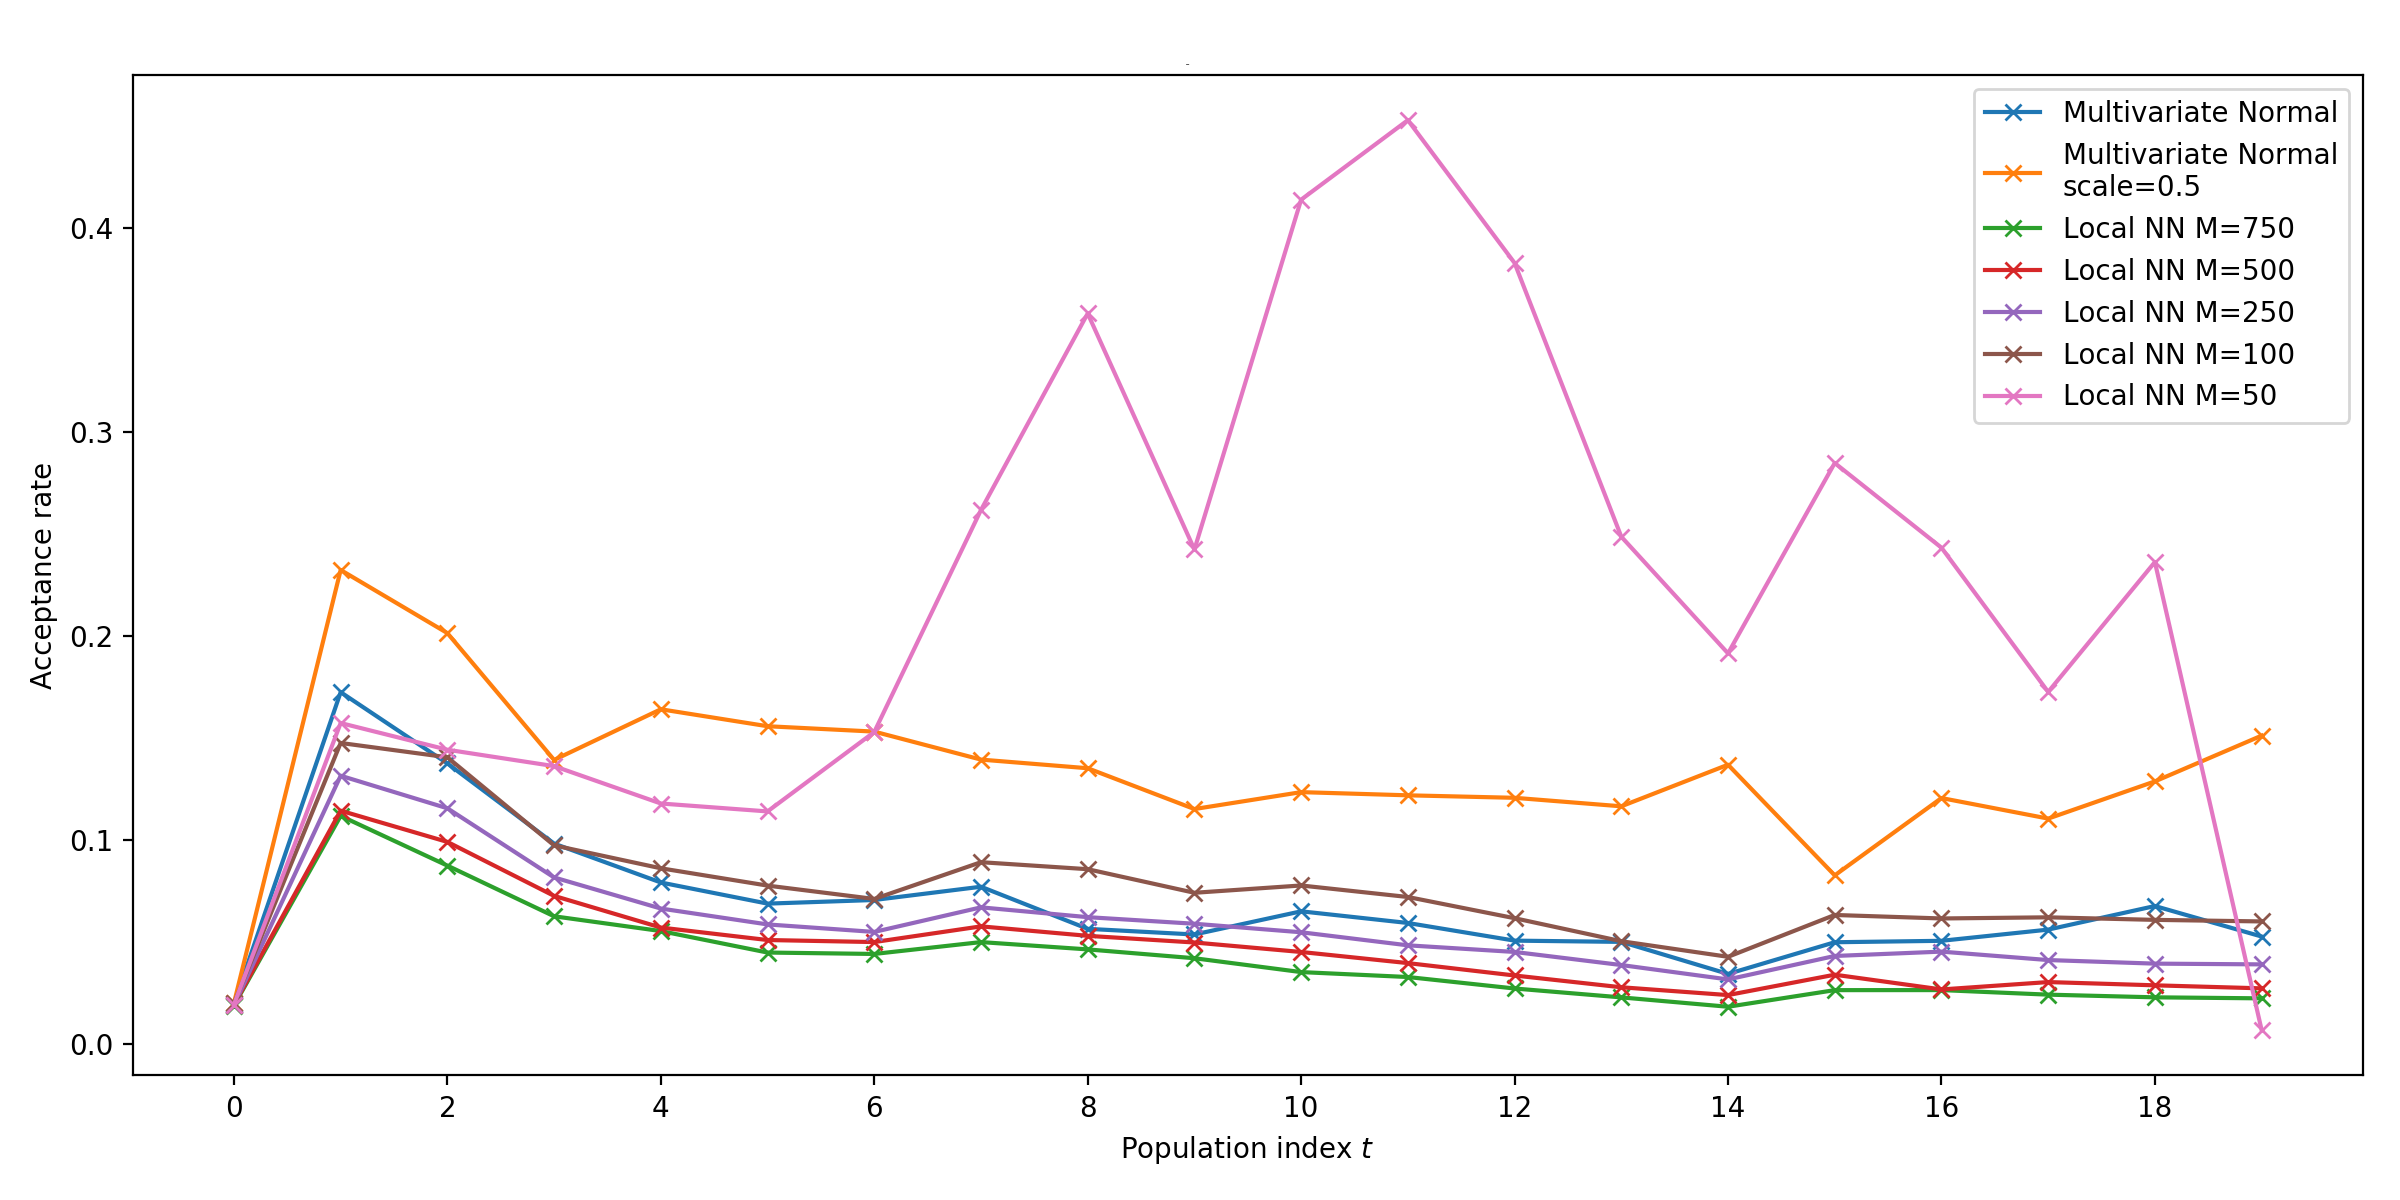
\includegraphics{fig/acceptance1.png}}
%     \end{center}

%     \caption{Acceptance rates of different kernels}
%     \label{fig:acceptance1}

% \end{figure}


\subsection{Adaptive functions and factors}

% [how adaptive distance work]

SMC can be more adaptive by introducing adaptive distance function and adaptive population; besides, factors can be applied to manually `normalise' the data.

The trivial distance function is set to Euclidean distance (2-norm distance)

\begin{align}
    \label{eq:dis}
    D=\sqrt{\sum_i \Delta x_i^2}
\end{align}

where $i$ is the index of data points and $\Delta x_i$ is the discrepancy between  observed data and simulated data at data point $i$, i.e. $\Delta x_i = x_{i, simulated}-x_{i, observed}$. In this case data points are 12 time points of four variables i.e. 48 data points in total.

A weighted 2-norm distance can be written as

\begin{align}
    \label{dis_w}
    D=\sqrt{\sum_i w_i \Delta x_i^2}
\end{align}

where a weight $w_i$ is assigned to every data point. If data point $i$ have a higher weight, then the data value is regeared to be more informative, i.e. giving more help in inferring the true posteriors; weights can be either pre-set according to prior knowledge of the problem, or using adaptive method to be dynamically calculated according to , known as adaptive distance.

Adaptive distance is changing the weights of all data points after each generation iteration, trying to assign informative data points higher weights. Additionally, implementation of adaptive in \verb|pyABC| also introduces additional factors $f_i$ multiplied to weights \cite{ref:adpt_dis}

\begin{align}
    \label{dis_f}
    D=\sqrt{\sum_i f_iw_i \Delta x_i^2}
\end{align}

Factor is helpful as an option for efficiency. When some data points are equally informative, the manually pre-defined can make the distance more focused on certain data point, or behave like a normalisation that can balance the scales of different summarised statistics (here is the 48 mean values). There are two appliance case studied: (1) factors used as an normalisation option and (2) factors used to give more focus on some features of the observed data. For (2), as we noticed that the main features (e.g. rapid increase, peaks, fluctuations) are mostly observed in the first half of the time points i.e. 0 - 30 hpl, factors are tried in the later parameter estimation of real data where a more accurate fit of the curve is desired.

Adaptive population \cite{population} can adapt the population size of each generation according to the mean correlation of variation error of the previous population. In our early test the maximal population size that is allowed is set to 5,000 and the adaptive strategy always select the upper bound, as a results of wide parameter space or the wide posterior approximation shape.

% [what is factor]

% [what is adaptive distance]

\subsubsection{Experiment results}

% [FIGURE here]

Two types of factor and adaptive distance function were tested by running the same number of generations (20 generation, 2000 particles per generation). The first type of factor is 25:75  factor, where first half of the trajectory data was assigned higher factor (75), and second half of the data was assigned lower factor (25); this could make the first half if the data more `important' in the inference. The second factor was range factor, which tried to normalise the trajectory of each dependent variable according to its data range.

From Figure \ref{fig:factor}, different types of factor gave different performance. 25:75 factor required much more samples in the first generation (orange bar in the left of Figure \ref{fig:factor}) and also did not improve much in later generations, thus it is the slowest one. The first half of observed data contained more features and information, assigning it with higher factor would make the algorithm think that it is more important to fit the first half and thus focus on the hard part, and consequently more particles were needed in the inference process. The acceptance rates of 25:75 factor among different generations were also generally slightly lower than the standard. By contrast, range factor required less total samples and gave generally higher acceptance rates than standard, which made it considerably faster. Adaptive distance gave the best efficiency, as it significantly improved the acceptance rates and resulted in even less required samples (right, Figure \ref{fig:factor}).

\begin{figure}[t!]
    \begin{center}
        \resizebox{1.0\hsize}{!}{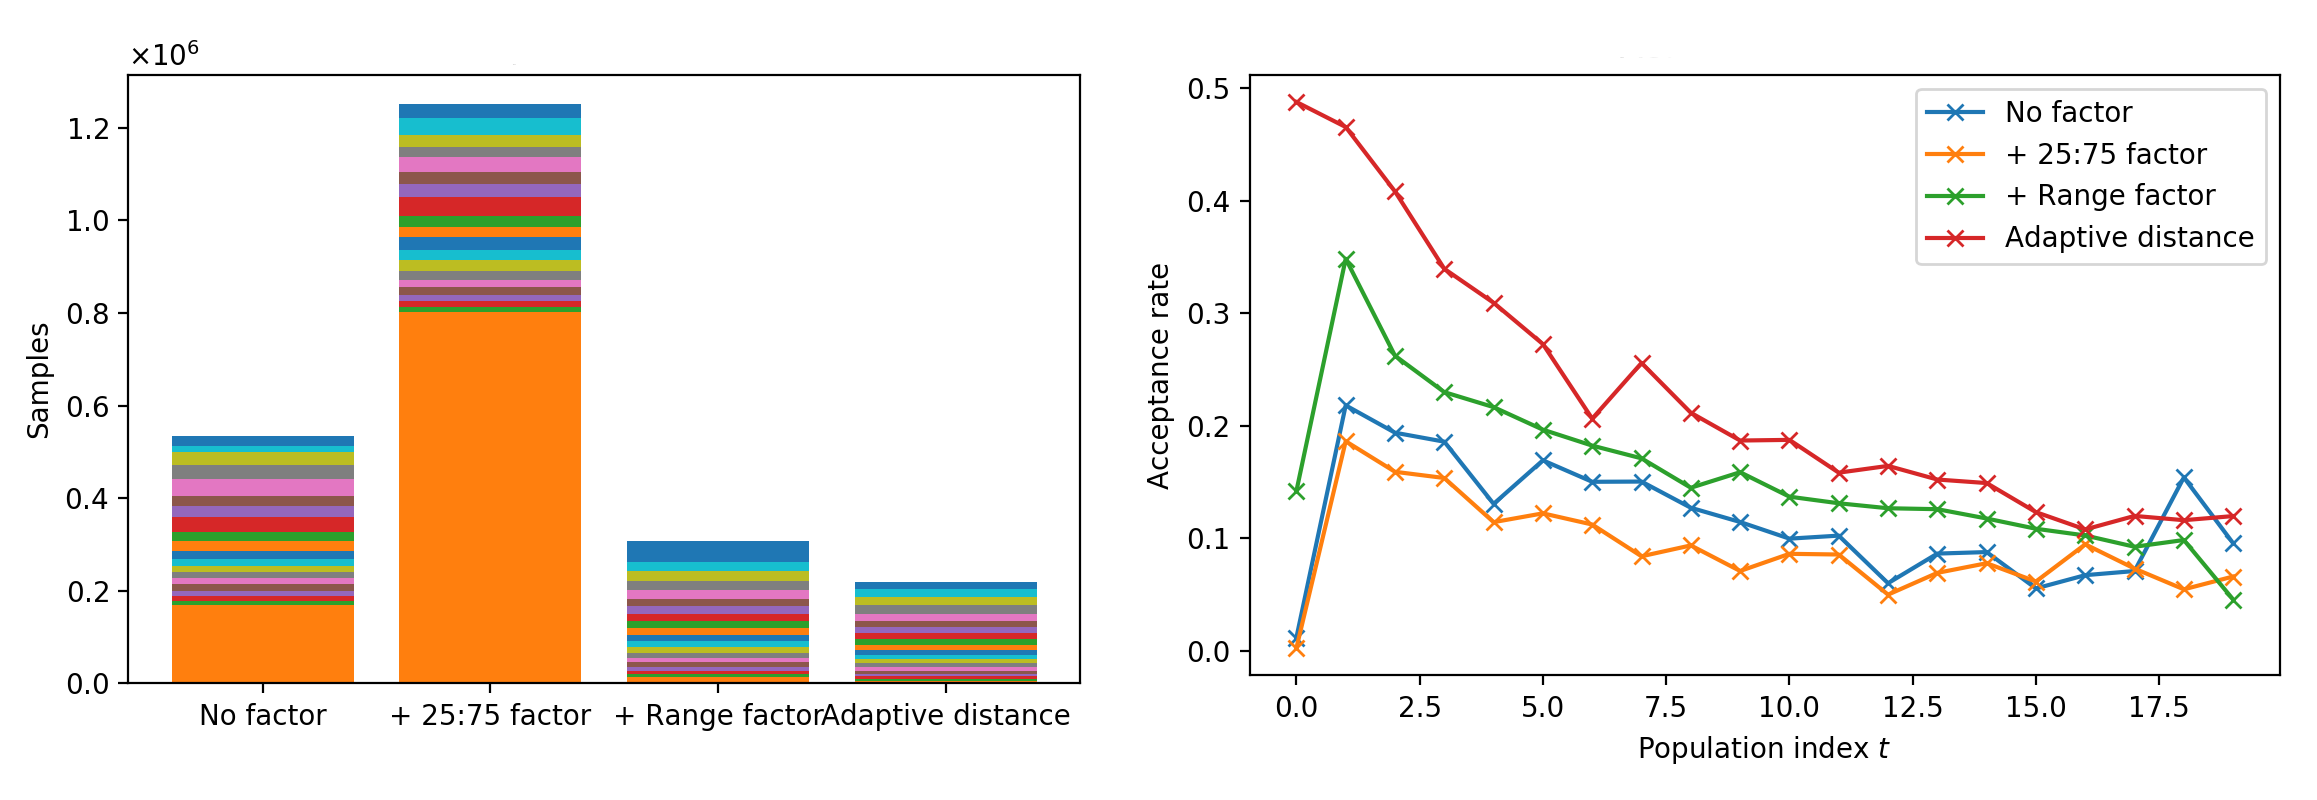
\includegraphics{fig/ib.png}}
    \end{center}

    \caption[Factors and adaptive distance experiments]%
    {Factors and adaptive distance experiments. Left: Total required samples. Right: acceptance rates in each generation}
    \label{fig:factor}

    \begin{center}
        \resizebox{1.0\hsize}{!}{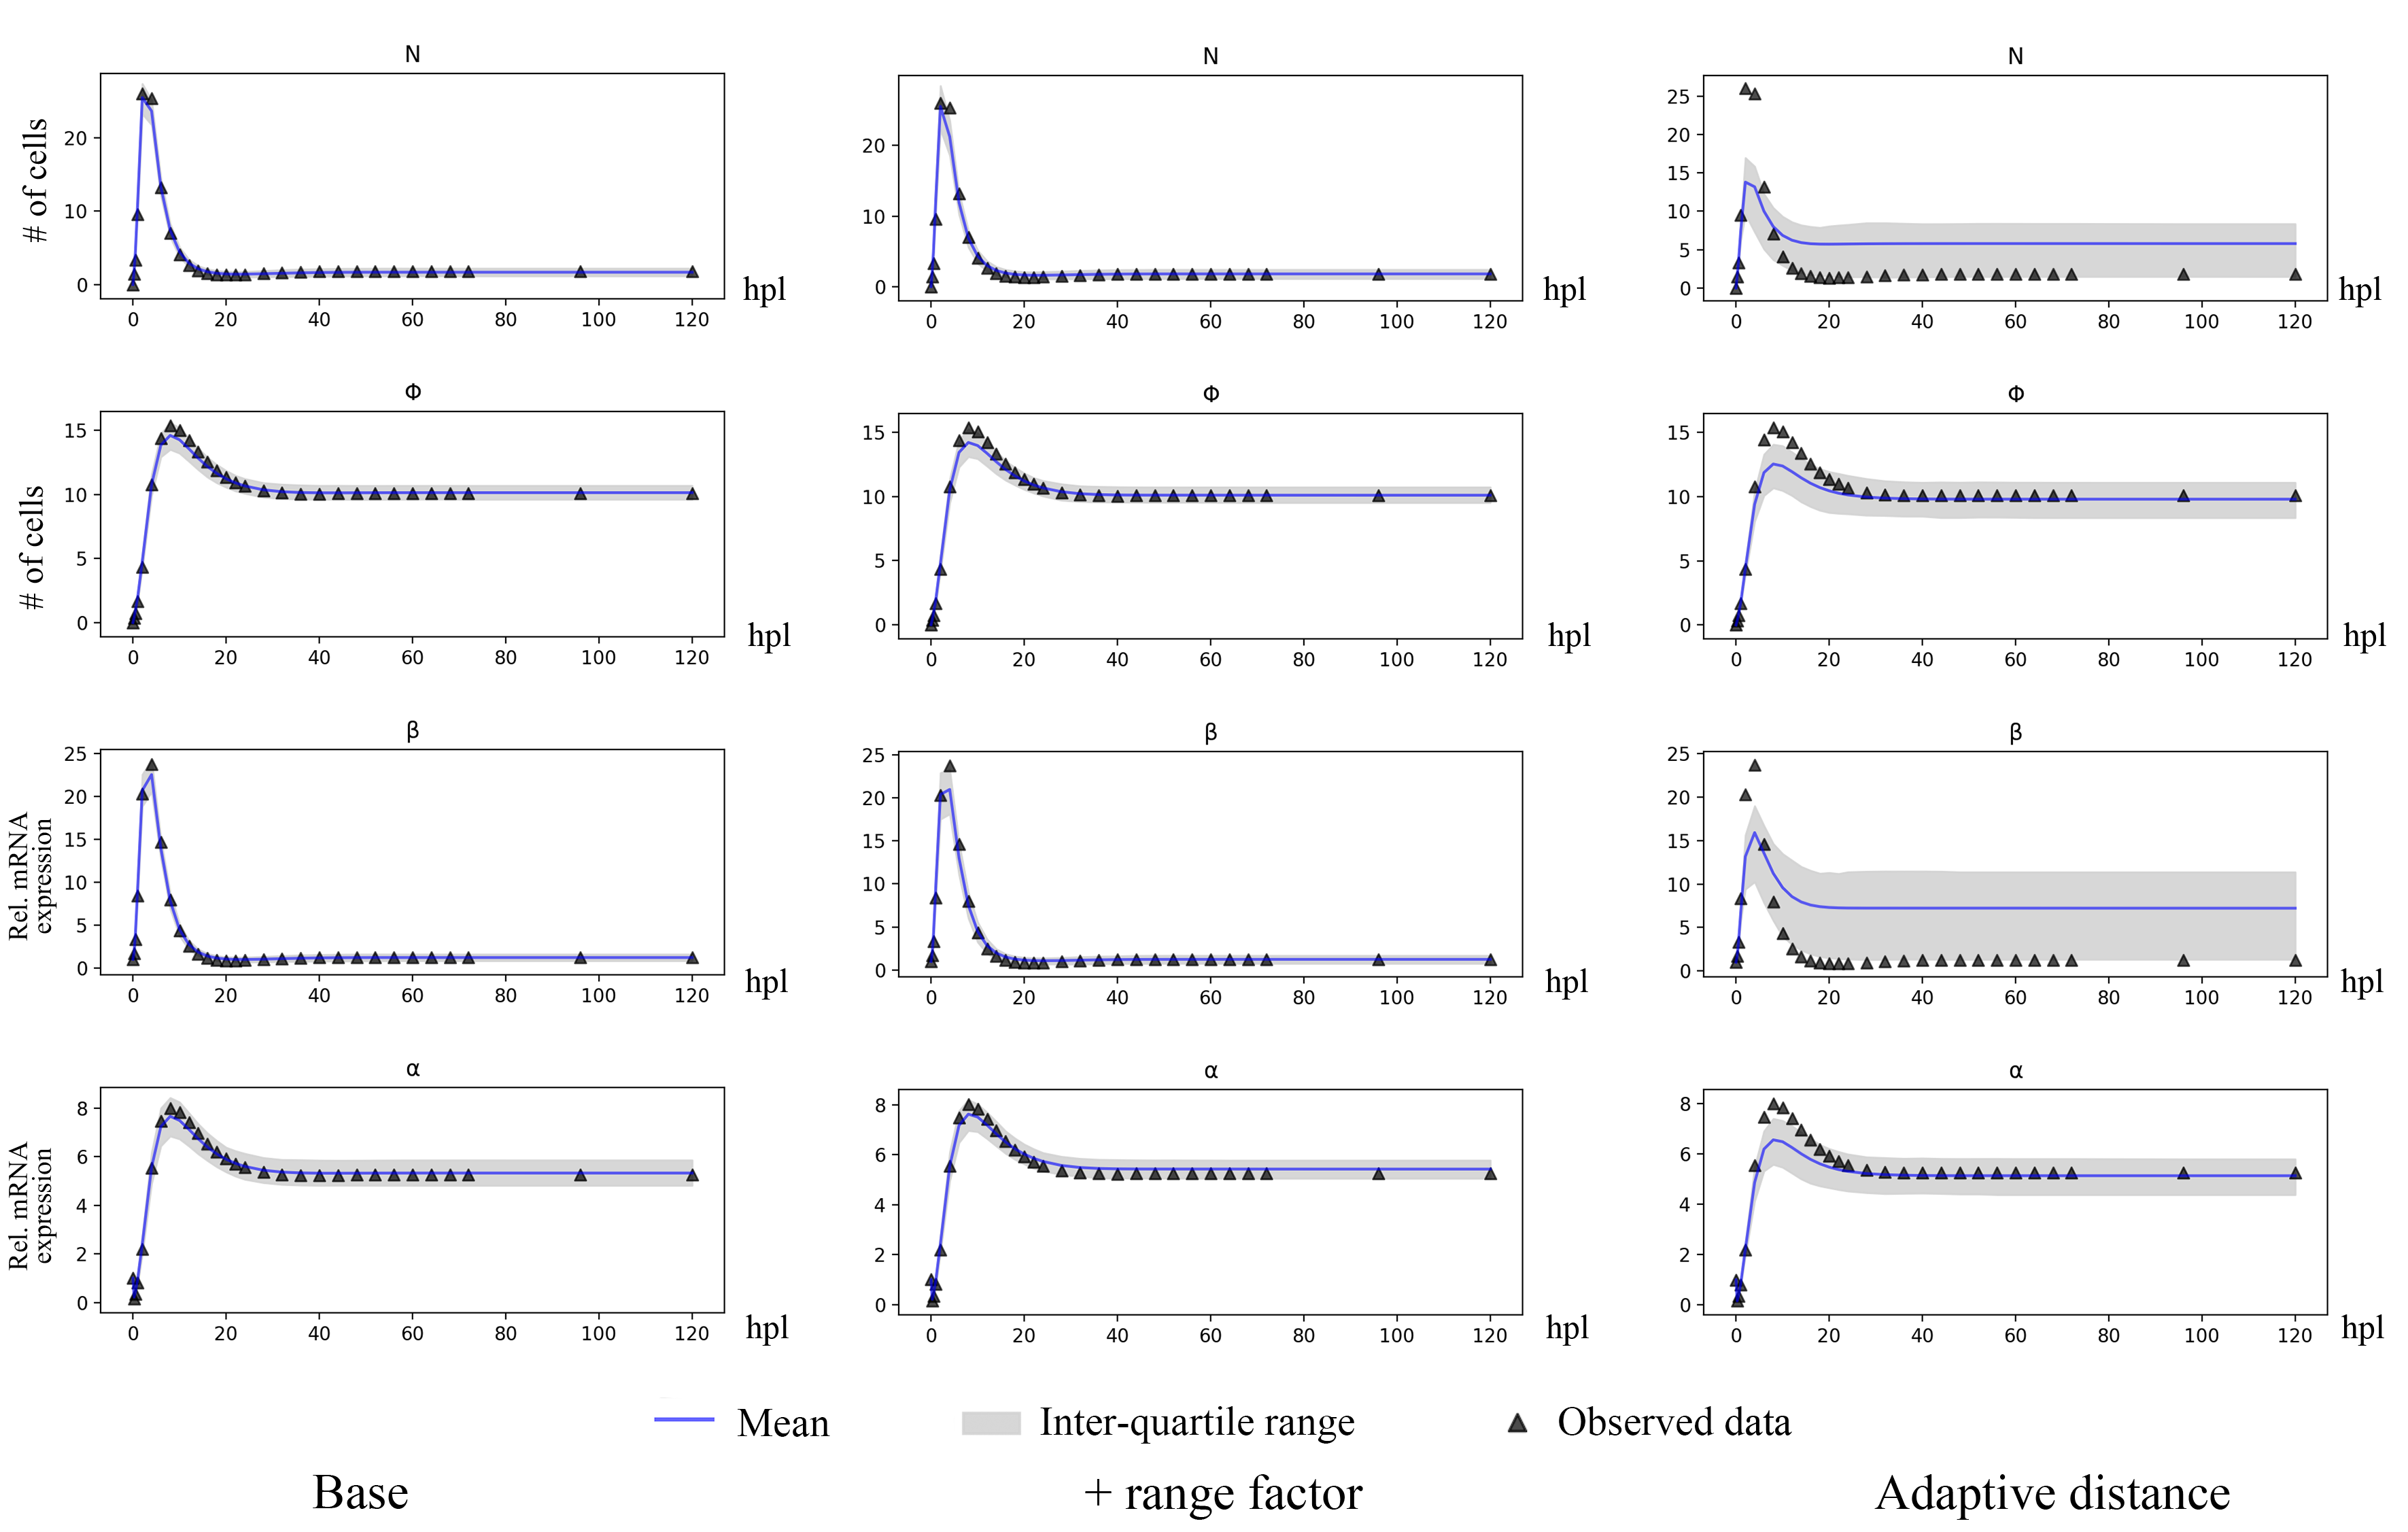
\includegraphics{fig/ib_factor.png}}
    \end{center}

    \caption[CAPTION]%
    {DESCRIBE}
    \label{fig:factor_sim}

\end{figure}

However, the result of factors adaptive distance could not be directly compared to standard run, because it changed the distance measurement by adapting weights or manually setting factors. Factors were normalise to make it more close the standard distance measurement. As a result, the same final threshold value did not guarantee that adaptive distance can reach the same level of fit as others. After 20 populations, adaptive distance had a poor fit (Figure \ref{fig:factor_sim}), while the standard run and two types of factors had similar tight fits of the data, which all converge to the true posterior. Additional in our implementations, variance factor (which tries to normalise the data according to the dependent variables' variance) was also tries and gave very similar performance as range factor.

To conclude, because the factors and weights are directly multiplied to $\Delta x$ and thus the metrics for distance are changed, the direct compare of the efficiency under the same threshold schedule was unfeasible; we could only compare the results after the same number of generations. Factors gave nearly the same inferred results but required different number of samples, hence cares must betaken when choosing factor schemes. Adaptive distance did not result in a accurate result as others. As a result, our further implementations used standard distance function, and factors were tried for possible improvements.


% by applying factors the total required samples are less, and the adaptive distance requires much less samples; their acceptance rates are also higher than the standard one. It seems that adaptive function and factors could help to converge more quickly.


% However considering the result after 20 generation (Figure \ref{fig:factor_sim}), the resultant model gives the contrary preference. Applying factors and using adaptive distance can lead the resultant model less accurate (after the same generation iterations): they have wider inter-quantile range and may requires more generations to converge. TODO

% \subsubsection{Conclusion} We noticed the significant efficiency improvement of these adaptive options; they can largely improve the acceptance rate in some cases. However, as the factors and weights are directly multiplied to $\Delta x$ and thus the metrics for distance are changed, a direct compare of the efficiency under the same threshold schedule is unfeasible; after the same number of generations they can reach a small $\epsilon_t$ but still the approximated posterior is not as accurate as the standard implementation. AS a result, our implementation of the parameter inference will only consider standard distance function and factors are only tested for improvements (FIGURE).


\subsection{Data size, prior distribution and population}

[experiments plan]

Some other hyperparameters, e.g. feed-in data size, prior distribution, number of populations and number of particles in each population were also of our interest. Experiments were designed to explore how these options affect the goodness of fit and efficiency of the implementation.

Regarding the existing dynamic systems model, SMC was applied with two data size options, three prior distribution (uniform distribution, wider uniform distribution and log-uniform distribution). The population options i.e. population size and number of populations were also tried with different values. These experiments intended to give suggestions on the later SMC implementation on experimental data.

\subsubsection{Experiments results}

The results from data size and prior distribution range is shown in FIGURE. The standard implementation is fed with 120 data points (30 data points for each of the four variables), the `less data' is fed with 48 data points, which is the case of the real experimental measurement. Although much less (60\%) data is used, the total required sampling numbers is not much less (XX\%). Although the data size does not affect the sampling process much and the inferred model are all considered acceptable when compared to the synthetic data (FIGURE), cares should be taken when using less data point, or using other more summative statistics, e.g. mean, standard deviation, peak values, starting and ending values etc. As shown in \cite{ref:disease}, less data can lead to a model with more variance, under-fitting or missing some local features e.g. local peak.

\begin{figure}[t!]
    \begin{center}
        \resizebox{1.0\hsize}{!}{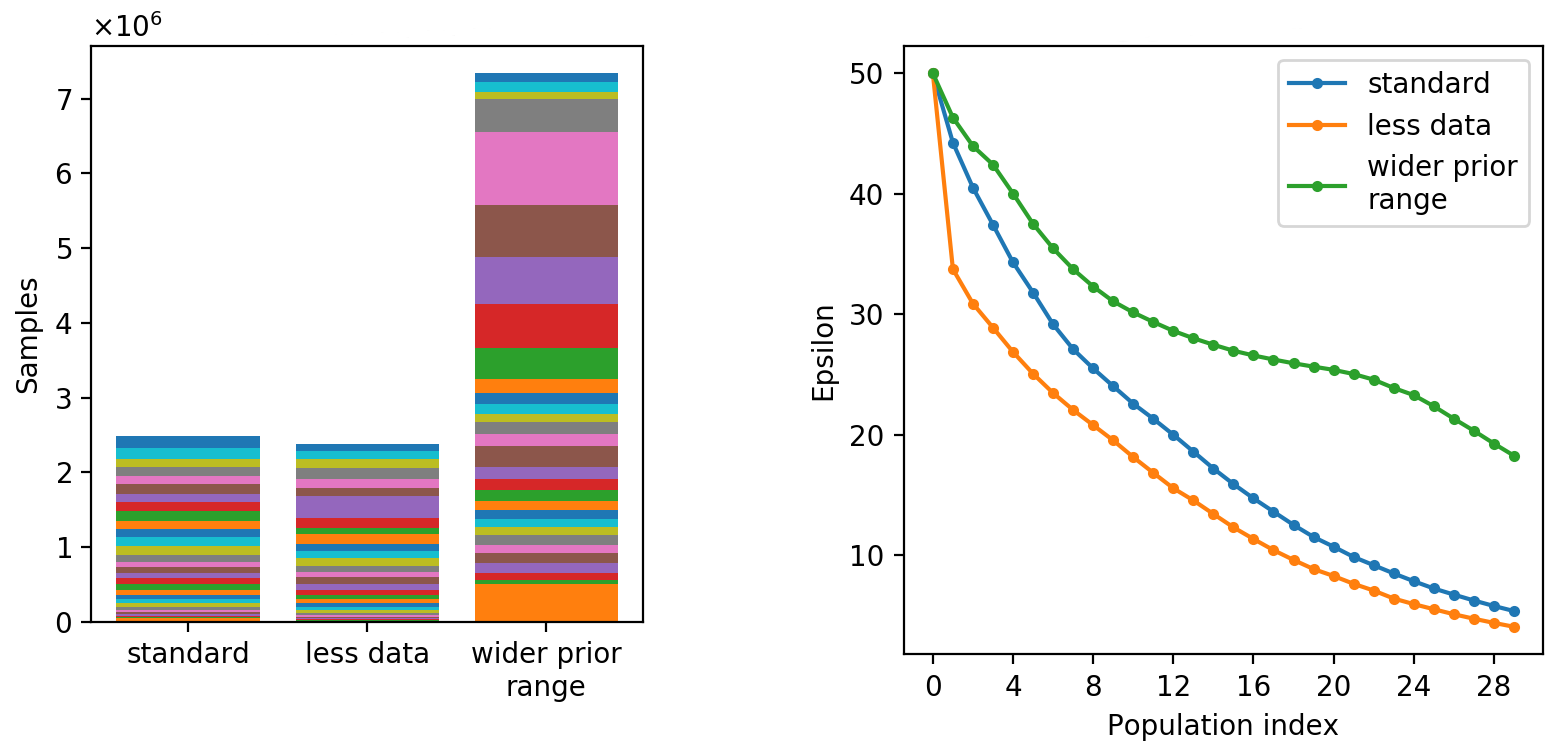
\includegraphics{fig/size1.png}}
    \end{center}

    \caption[Data size and prior distribution range experiment]%
    {Data size and prior distribution range experiment. (a) Total required samples, (b) Epsilon values under median epsilon schedule}
    \label{fig:size}

\end{figure}

The prior range and distribution can largely affect the execution of SMC (FIGURE and FIGURE). Samples are taken from a high dimensional parameter space in each sampling process, wider prior distribution ranges will making each sampling explore more in the parameter vector space. It suggests that a narrower prior is preferred and we should make a more accurate and confident prior belief as possible for the efficiency concerns.

%     [discuss uniform and log uniform when result ready]

% [FIGURE HERE]


\subsubsection{Summary} This subsection aims to preliminarily explore ABC SMC settings using synthetic data with known true parameter values, thus the efficiency and the goodness of the resultant model can be compared across these options. Conclusion can be drawn to choose efficient and proper options of ABC SMC to be applied on the target models with experimental data. It also provides reference for a general inference task using SMC with high dimensional parameter space.








\section{Parameter estimation and model comparison}

\subsection{Model 1, 2 and 3}

[separated ABC run on model 1, 2 and 3]

Using the suggested options in the previous section, the target data (Figure \ref{fig:obs_data}) is prepared as input for the SMC inference framework. Regarding the result, the population size and number of generations are adjusted several times to obtain an general informative posterior which should be stable across repeated runs and avoid local optimal as much as possible.

Parameter estimation of model 1, 2 and 3 was tried with different prior distribution setting: distribution range [0, 25] and [0, 75], amd distribution type uniform and log-uniform. All these ABC SMC runs uses 2,000 particles per population and 30 generations.

Log-uniform-shaped prior seems to give a better fit of the model, and wider prior range [0, 75] does not give a more accurate result. Then distribution range [0, 25] was tried, in case some parameter have a true posterior laying between [25, 50].

The results of prior distribution log-uniform [0, 50] is shown in Figure \ref{fig:result123}. For model 3, the acceptance rates and epsilon path are presented in Figure \ref{fig:result123_2}. For model 3, the estimated parameters' posterior is shown in Figure \ref{fig:para1}. Figure \ref{fig:result123} plots the estimated curve of models, using the mean value of each parameter's approximated posterior; also 1000 particles (each particle is a parameter set) were sampled and used to generate simulated trajectories of the four variable, and the mean (blue) and 25th to 75th percentile range (grey) are calculated from the 1000 simulated data.

Before applying model comparison methods, some features of the three model can still be compared. From simulated curves, It can be seen that all the inter-quartile ranges are tight around the mean value curve, which indicates the approximated posterior are concentrated to some degree; the peak-shaped posterior distributions (Figure \ref{fig:para1}) agrees with this. All epsilon values converges to a steady level, and model 3 has a lower final epsilon value and consequently the simulated trajectory is more close to the observed data (model 3, Figure \ref{fig:result123}).

The acceptance rates is fluctuating and have a gradually increase trend for all the three models, as the acceptance rate becomes higher when the true posteriors are gradually approximated. Compared to model 1, model 2 gives a better fit of the decreasing trend at the second half of the observed data, by using a exponentially decaying self-increase rate $\lambda_N$ instead of a constant. The resultant simulated data from model 2 and 3 are in the similar trends and the most obvious difference is that for model 3, the simulated data of $\Phi$ and $\alpha$ are more `flat'. We expect model 3 to be the best model as it reaches a threshold value and intuitively gives a better fit, although the fit could not be considered generally a good representation of the biological process that we want to model, as the simulated data are significantly biased from the observed data for tnf-$\alpha$. A sharp peak at 4 hpl is observed from the measurement (Figure \ref{fig:obs_data}) but no similar features are represented by any of the three models.

\begin{figure}
    \begin{center}
        \resizebox{1.0\hsize}{!}{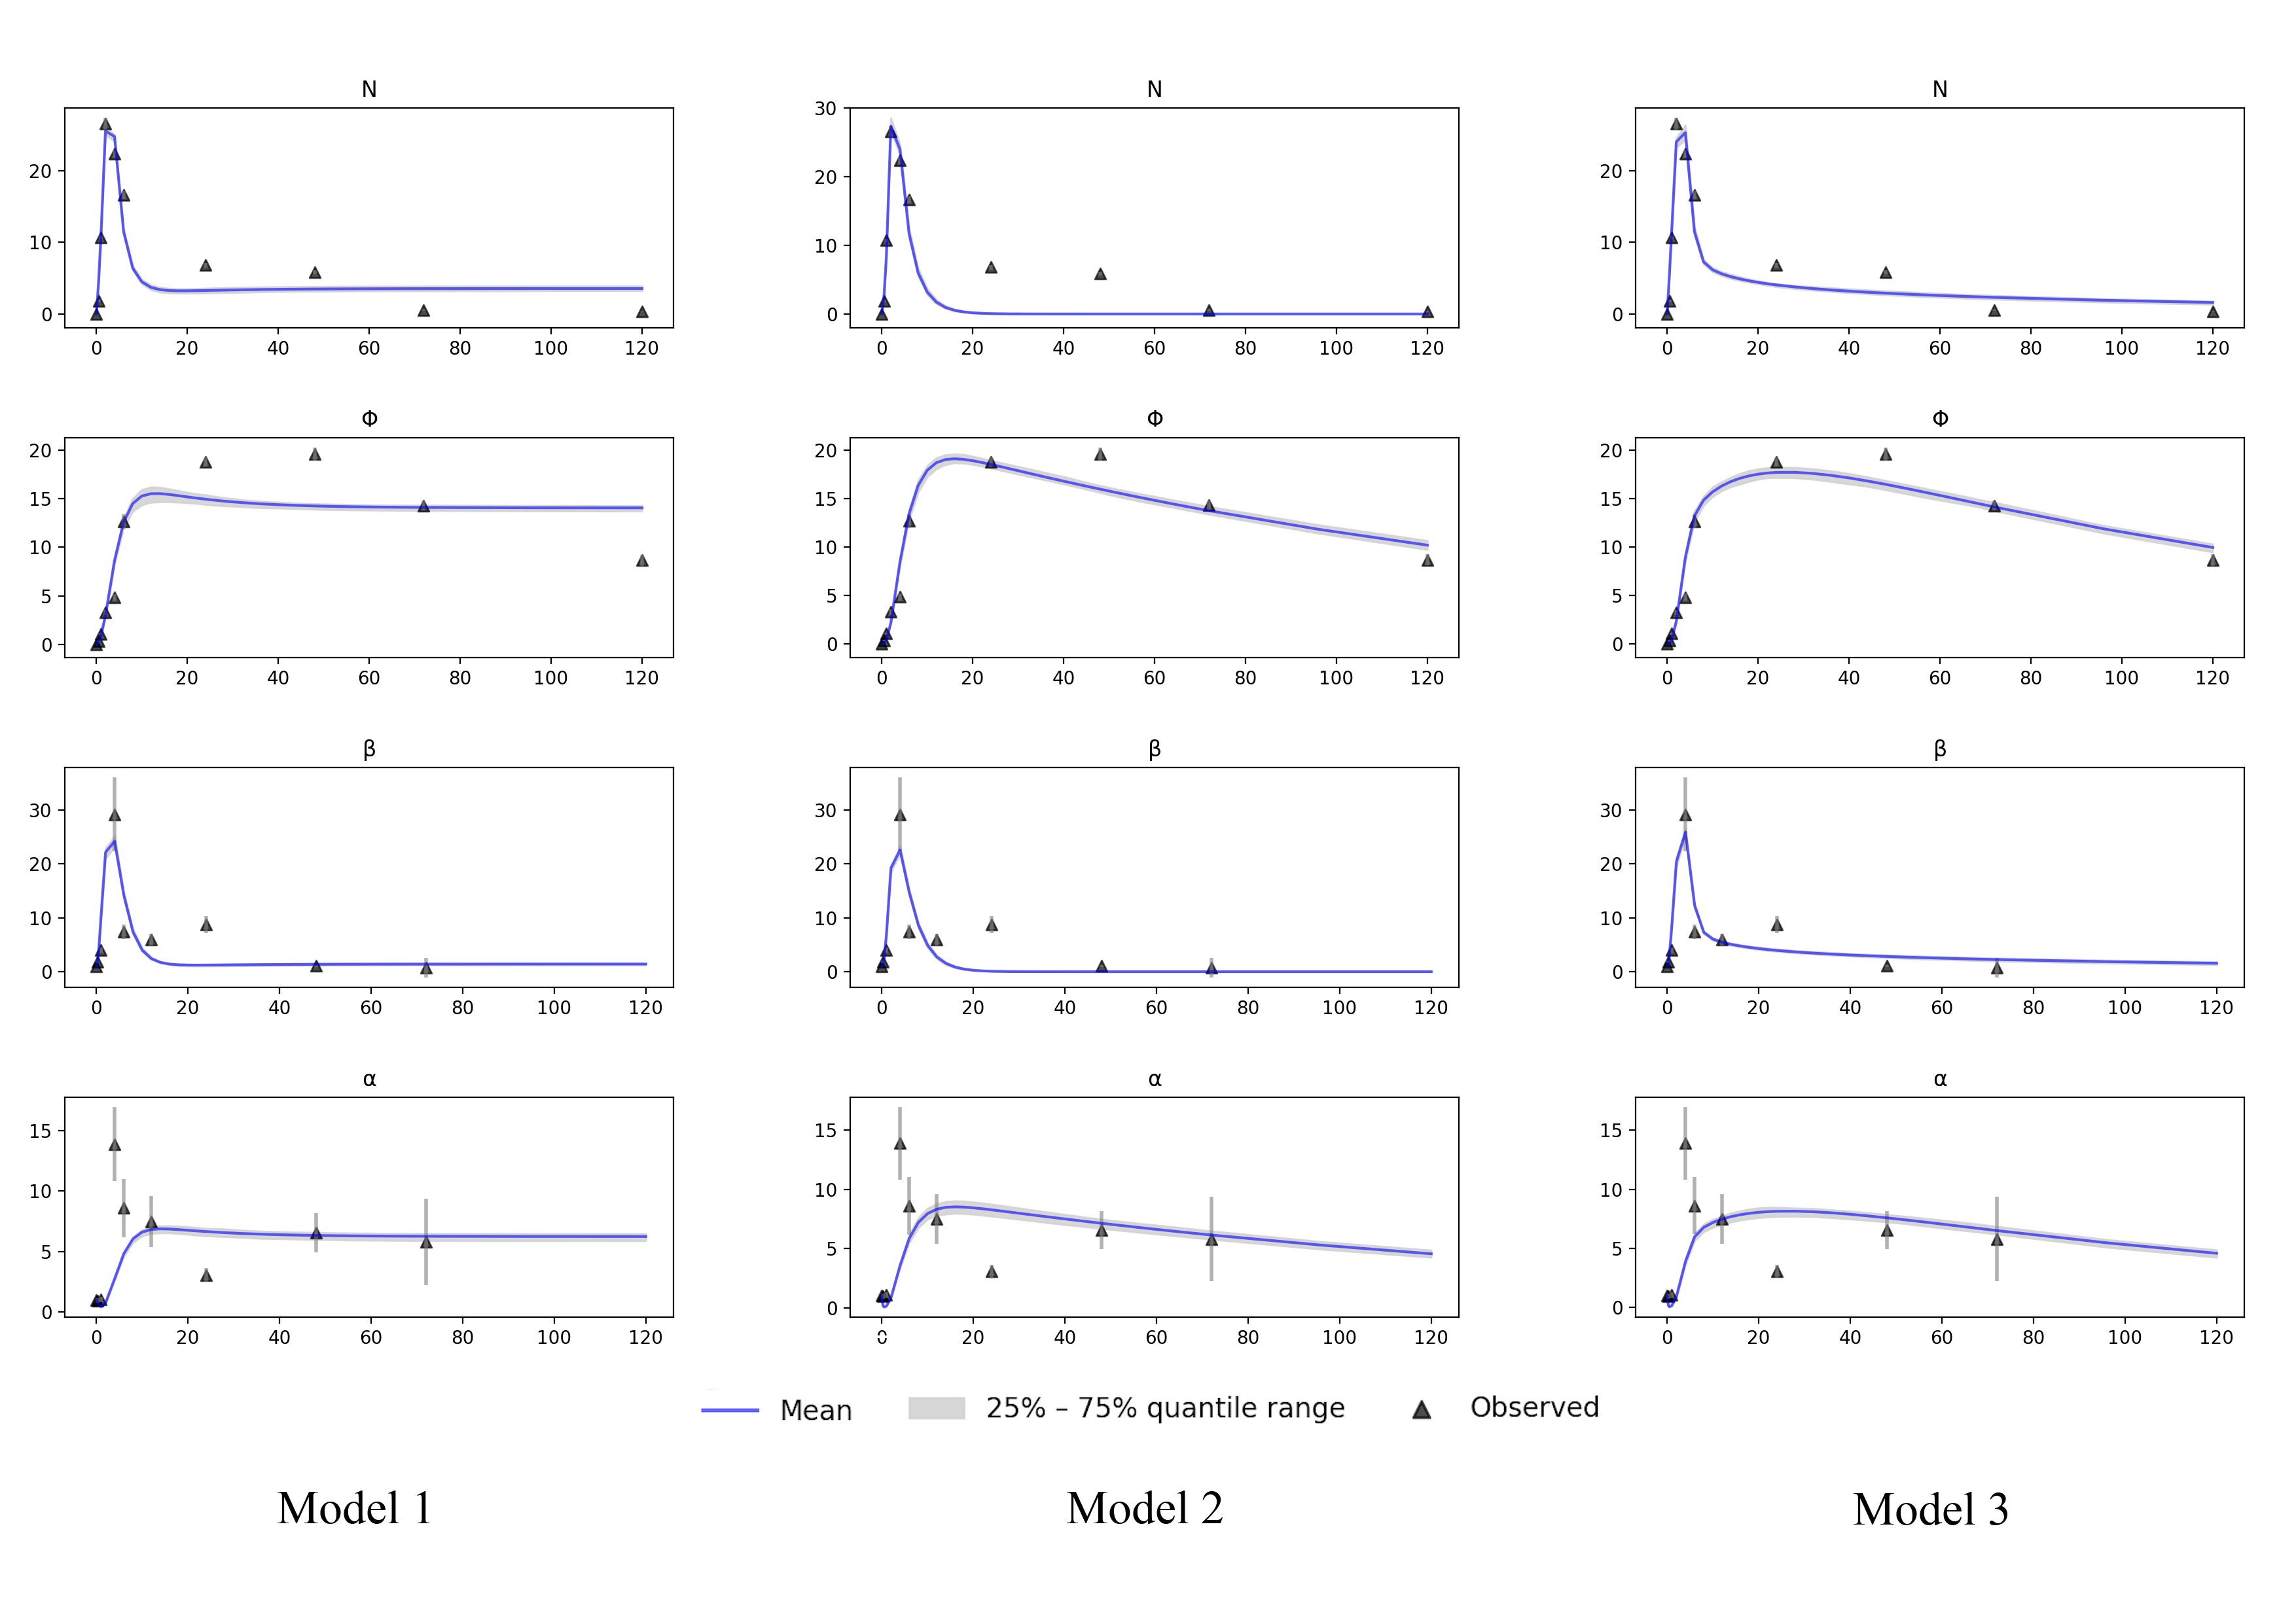
\includegraphics{fig/resultCurve123.png}}
    \end{center}

    \caption[Simulated trajectory from the 20th population of model 1, 2 and 3]%
    {Simulated trajectory from the last population of model 1, 2 and 3. Error bar indicates SEM. 500 randomly chosen particles from last population are used to generate a sequence of trajectories where mean and inter-quartile range are calculated from}
    \label{fig:result123}


    \vspace*{\floatsep}


    \begin{center}
        \resizebox{0.6\hsize}{!}{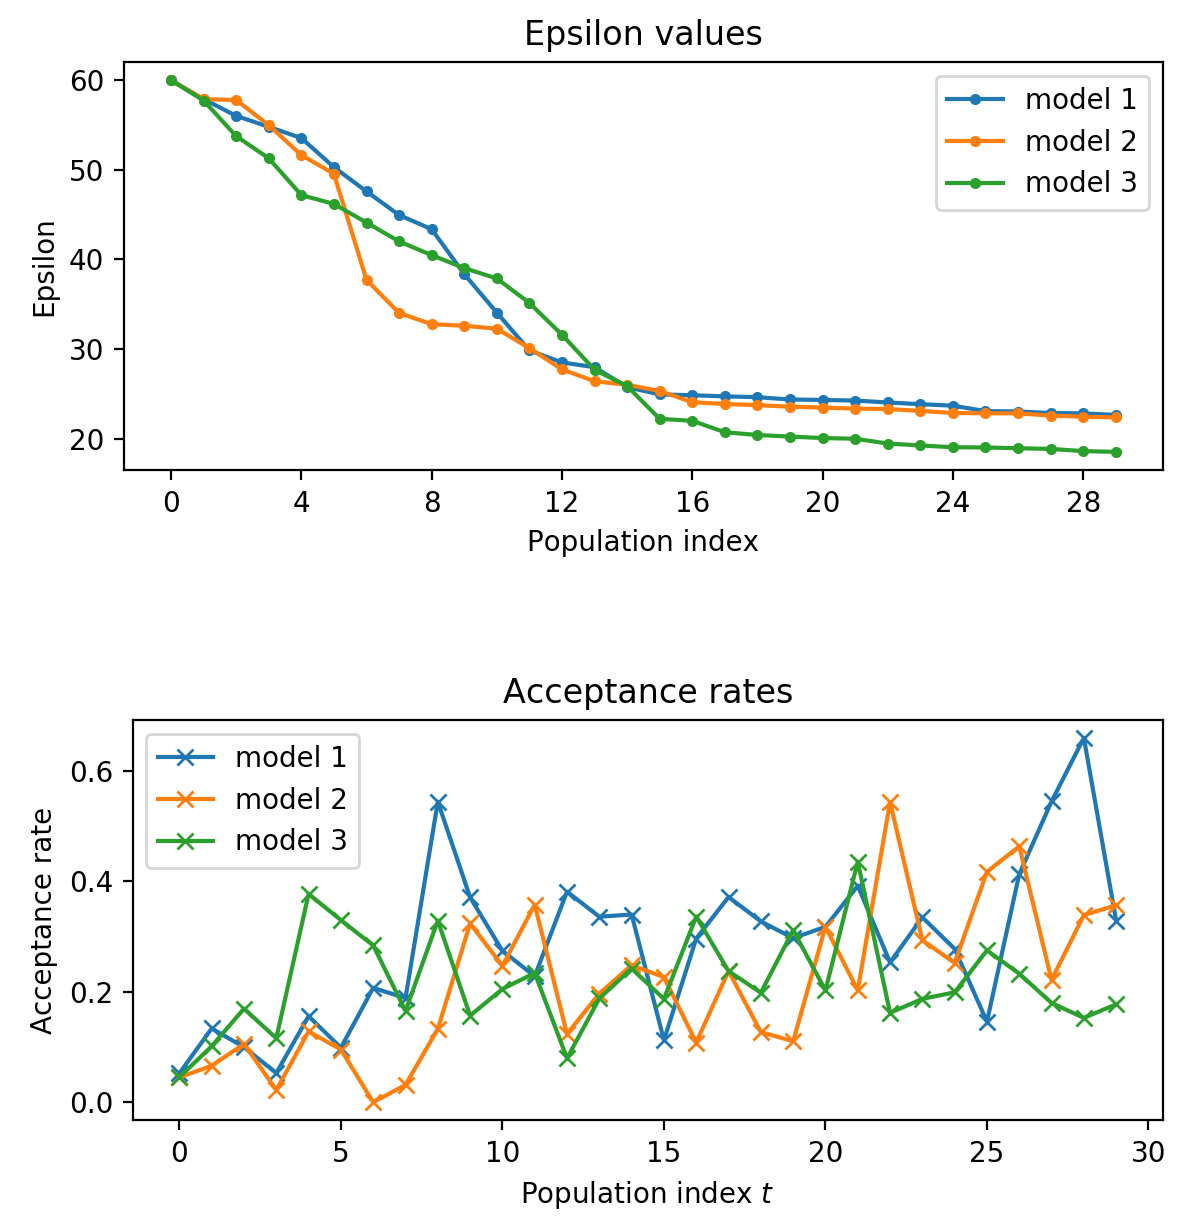
\includegraphics{fig/eps_acc123.png}}
    \end{center}

    \caption{Epsilon trends and acceptance rates of model 1, 2 and 3}
    \label{fig:result123_2}

\end{figure}

\begin{figure}
    \begin{center}
        \resizebox{1.0\hsize}{!}{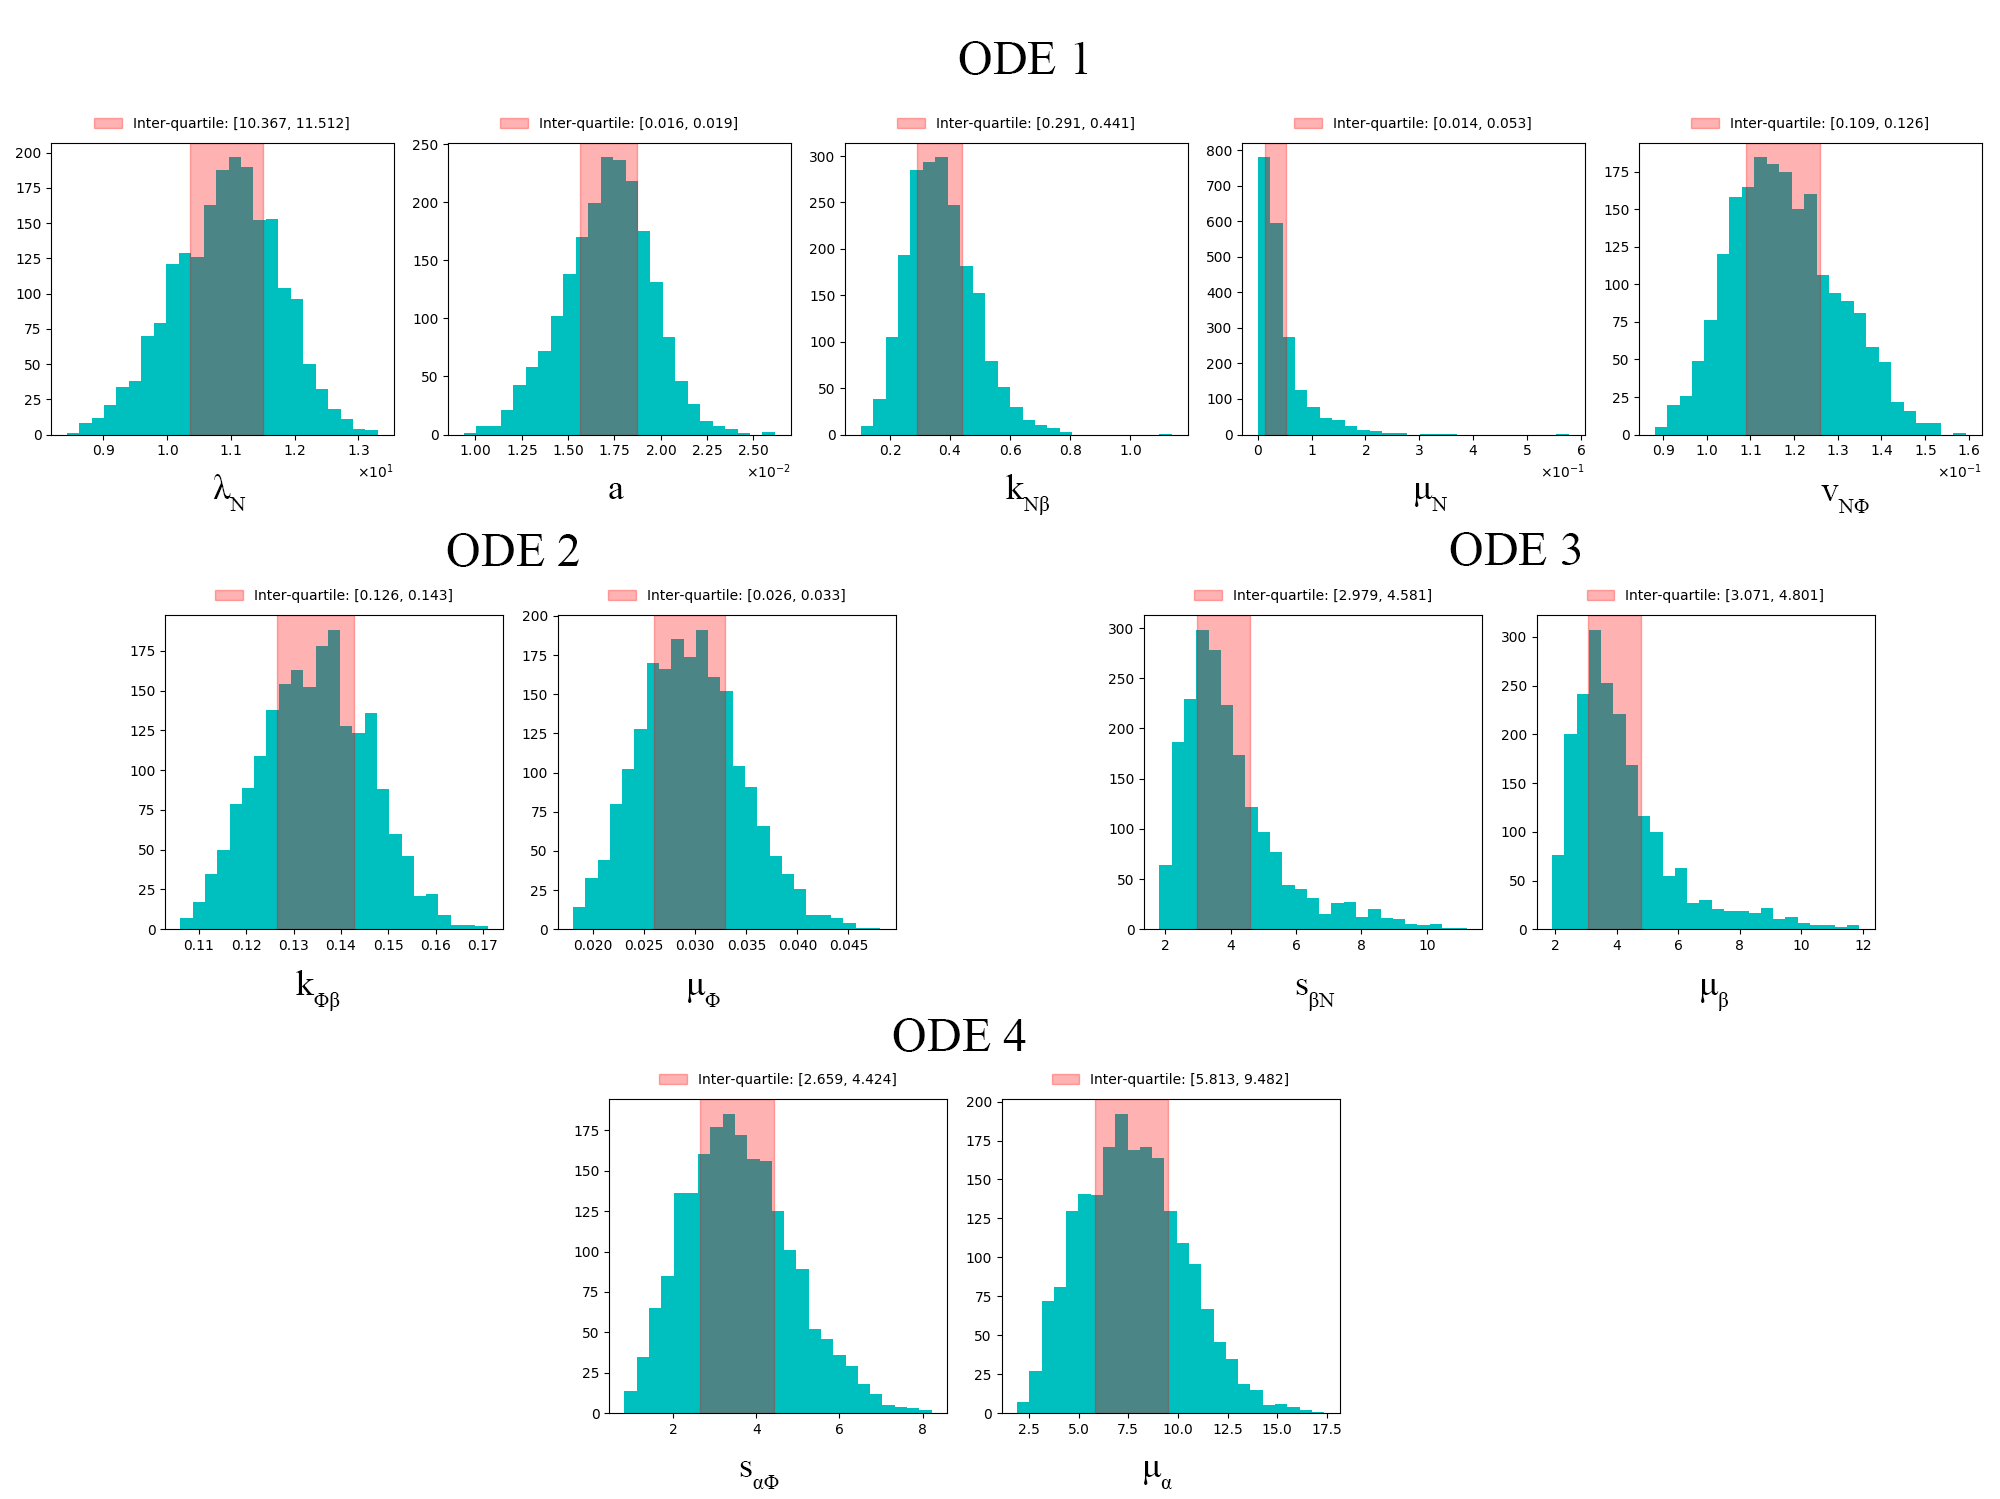
\includegraphics{fig/para1234.png}}
    \end{center}

    \caption[Estimated posterior distribution of parameters in model 3]%
    {Estimated posterior distribution of parameters in model 3. Shaded range indicates 25\%--75\% quantile of the population}
    \label{fig:para1}

    \begin{center}
        \resizebox{1.0\hsize}{!}{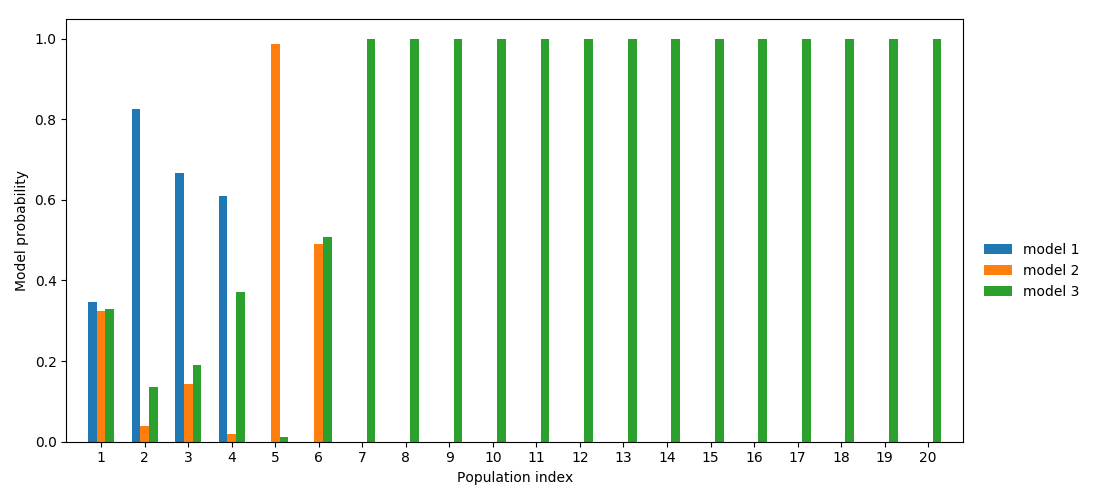
\includegraphics{fig/cmp1.png}}
    \end{center}

    \caption[ABC SMC based model comparison of model 1, 2 and 3]%
    {ABC SMC based model comparison of model 1, 2 and 3. From population 8 to population 30, model3 always wins}
    \label{fig:cmp1}

\end{figure}

[model comparison among model 1, 2, 3]

Next a model selection experiment with different prior was conducted, using the same ABC-SMC framework. As in the parameter inference, two distributions (uniform and log-uniform) are tested with three different interval ([0, 25], [0, 50] and [0, 75]). The results show that model 3 wins with nearly 100\% model probability at most runs after 30 generations, except log-uniform [0, 75]. All the model probability results are of great discrepancy (e.g. 100\% model 3 and 0\% for model 1 and 2), so Bayesian factor is not calculated.

Figure \ref{fig:cmp1} shows the model selection process, under log-uniform [0, 50] prior distribution. Model 3 gains total advantage over model 1 and 2 after 7th population. Together with conclusions above, model 3 is considered to be the the best model to represent the target data so far.



\begin{table}[t!]
    \centering
    \begin{tabular}{|c c c|}
        \hline
        Parameter            & Estimated mean  & Estimated mean      \\
                             & value (uniform) & value (log-uniform) \\[0.5ex]
        \hline\hline
        $\lambda_N$          & 14.1            & 13.3                \\
        $a$                  & 9.67            & 0.0170              \\
        $\kappa_{N\beta}$    & 18.0            & 0.259               \\
        $\mu_N$              & 13.2            & 0.0180              \\
        $\nu_{N\Phi}$        & 0.742           & 0.131               \\
        \hline
        $\kappa_{\Phi\beta}$ & 0.239           & 0.156               \\
        $\mu_\Phi$           & 0.154           & 0.0350              \\
        \hline
        $s_{\beta N}$        & 6.75            & 1.21                \\
        $\mu_\beta$          & 6.38            & 1.32                \\
        \hline
        $s_{\alpha\Phi}$     & 17.0            & 5.83                \\
        $\mu_\alpha$         & 11.9            & 2.43                \\
        \hline
    \end{tabular}
    \caption[Estimated parameter values of model 3]
    {Estimated parameter values of model 3, using uniform prior distribution and log-uniform prior distribution respectively}
    \label{table:estimated1}
\end{table}

Compared to uniform distributed prior, we found that log-uniform distributed prior is more suitable in the inference. Log-uniform results in an obviously better fit and narrower inter-quantile interval (Figure \ref{fig:result123} and \ref{fig:resultCurve_uni}), and the final epsilon value is also smaller. Log-uniform tends to assign values that are close to the left boundary (i.e. zero in our case) higher density, i.e. they are more likely to be sampled in the first population. As a result, the estimated parameter posteriors are expected to have smaller mean and/or skewed to left of the x-axis. The estimated values proved this (see \ref{table:estimated1}; also observed in other models and prior interval experiments). It indicates that some of the true parameter tend to have small values that are close to zero, and using log-uniform distribution could results in a faster and more satisfying inference. Regarding this, further experiments all use log-uniform distribution only.


\subsection{Model 4 and 5}

[features that derive model 4 and 5]

We observed that the existing models cannot well represent the trajectory of relative expression of tnf-$\alpha$: from experimental data, a rapid increase of tnf-$\alpha$ expression is observed in 0--4 hpl, followed by a rapid drop; all the models cannot well recover this feature and most test results see a less-rapid increase followed by a gradually decree and the observed peak value is not reached (e.g. Figure \ref{fig:result123}). Also in some other case e.g. Figure \ref{fig:resultCurve_uni}, tnf-$\alpha$ trajectories is well fitted at the cost of under-fitting $\Phi$. Hence efforts had been spent to propose more alternative models that can possibly solve this problem.

The two proposed alternative models is based on model 3 and try to add extra term in the tnf-$\alpha$ equation $\mathrm{d} \alpha/\mathrm{d} t$. As macrophage is the main source of tnf-$\alpha$ production, and a similar sharp increase-and-drop trend is observed in the il-1$\beta$ trajectory, two hypothesis and corresponding terms are propose as follows.

\paragraph{Model 4} It is assumed that the expression of il-1$\beta$ would have a promoting effect, representing by a phenomenological term $d_{\beta\alpha}\beta$ and $d_{\beta\alpha}$ is a new model parameter (positive constant). The promoting effect here is regarded to have the equivalent effect as directly promoting by il-1$\beta$, but the underlying mechanism is unclear so far. In mathematical view, this additional term can accelerate the expression of tnf-$\alpha$ in the first few time points and help to recover the peak-shaped trajectory. The proposed model is written as Equation \ref{eq:model4}.

\paragraph{Model 5} Alternatively, we considered promotions to the tnf-$\alpha$ production, i.e. $s_{\alpha\Phi}\Phi$. It is assumed that il-$\beta$ could accelerate the production process. An additional term $f_{\beta\alpha}\beta$ is introduced to production rate, with $f_{\beta\alpha}$ being a new model parameter (positive constant). This model meets the biological context considering the source of tnf-$\alpha$. The proposed model is written as Equation \ref{eq:model5}.

[further comparison of model 3, 4 and 5]

Model 4 and 5 are base on model 3, so in this phase experiments of these three models are conducted for separately parameter inference and overall model comparison. Based on our experience in conducted experiments, we used the following setting for parameter inference:

\begin{itemize}
    \item population size: 2000 and 5000
    \item number of populations: 30 generations
    \item prior: [0, 50] log-uniform
    \item perturbation kernel: multivariate normal kernel
\end{itemize}

Factors (Equation \ref{dis_f}) are also tried to find if we can force the inference framework to give more importance on the first few data points. In this experiment, for each trajectory first 8 data points are assigned higher factors (0.75), and the rest 4 data points are assigned with lower factors (0.25). All these runs are conducted on remote machines and the output database files are retrieved form analysis.

Figure \ref{fig:resultCurve345} shows the simulated data from the inferred models, with population size 2000. It can be seen that the addressed problem in the trajectory of tnf-$\alpha$ is partially relieved in model 4 and 5: compared to model 3, a peak appears around 4 hpl; it can represent more features in the observed data and consequently the final reached epsilon (after 30 populations) is smaller than that of model 3, which proves that our proposed modifications in model 4 and 5 are helpful in recovering more features in observed data.

\begin{figure}
    \begin{center}
        \resizebox{1.0\hsize}{!}{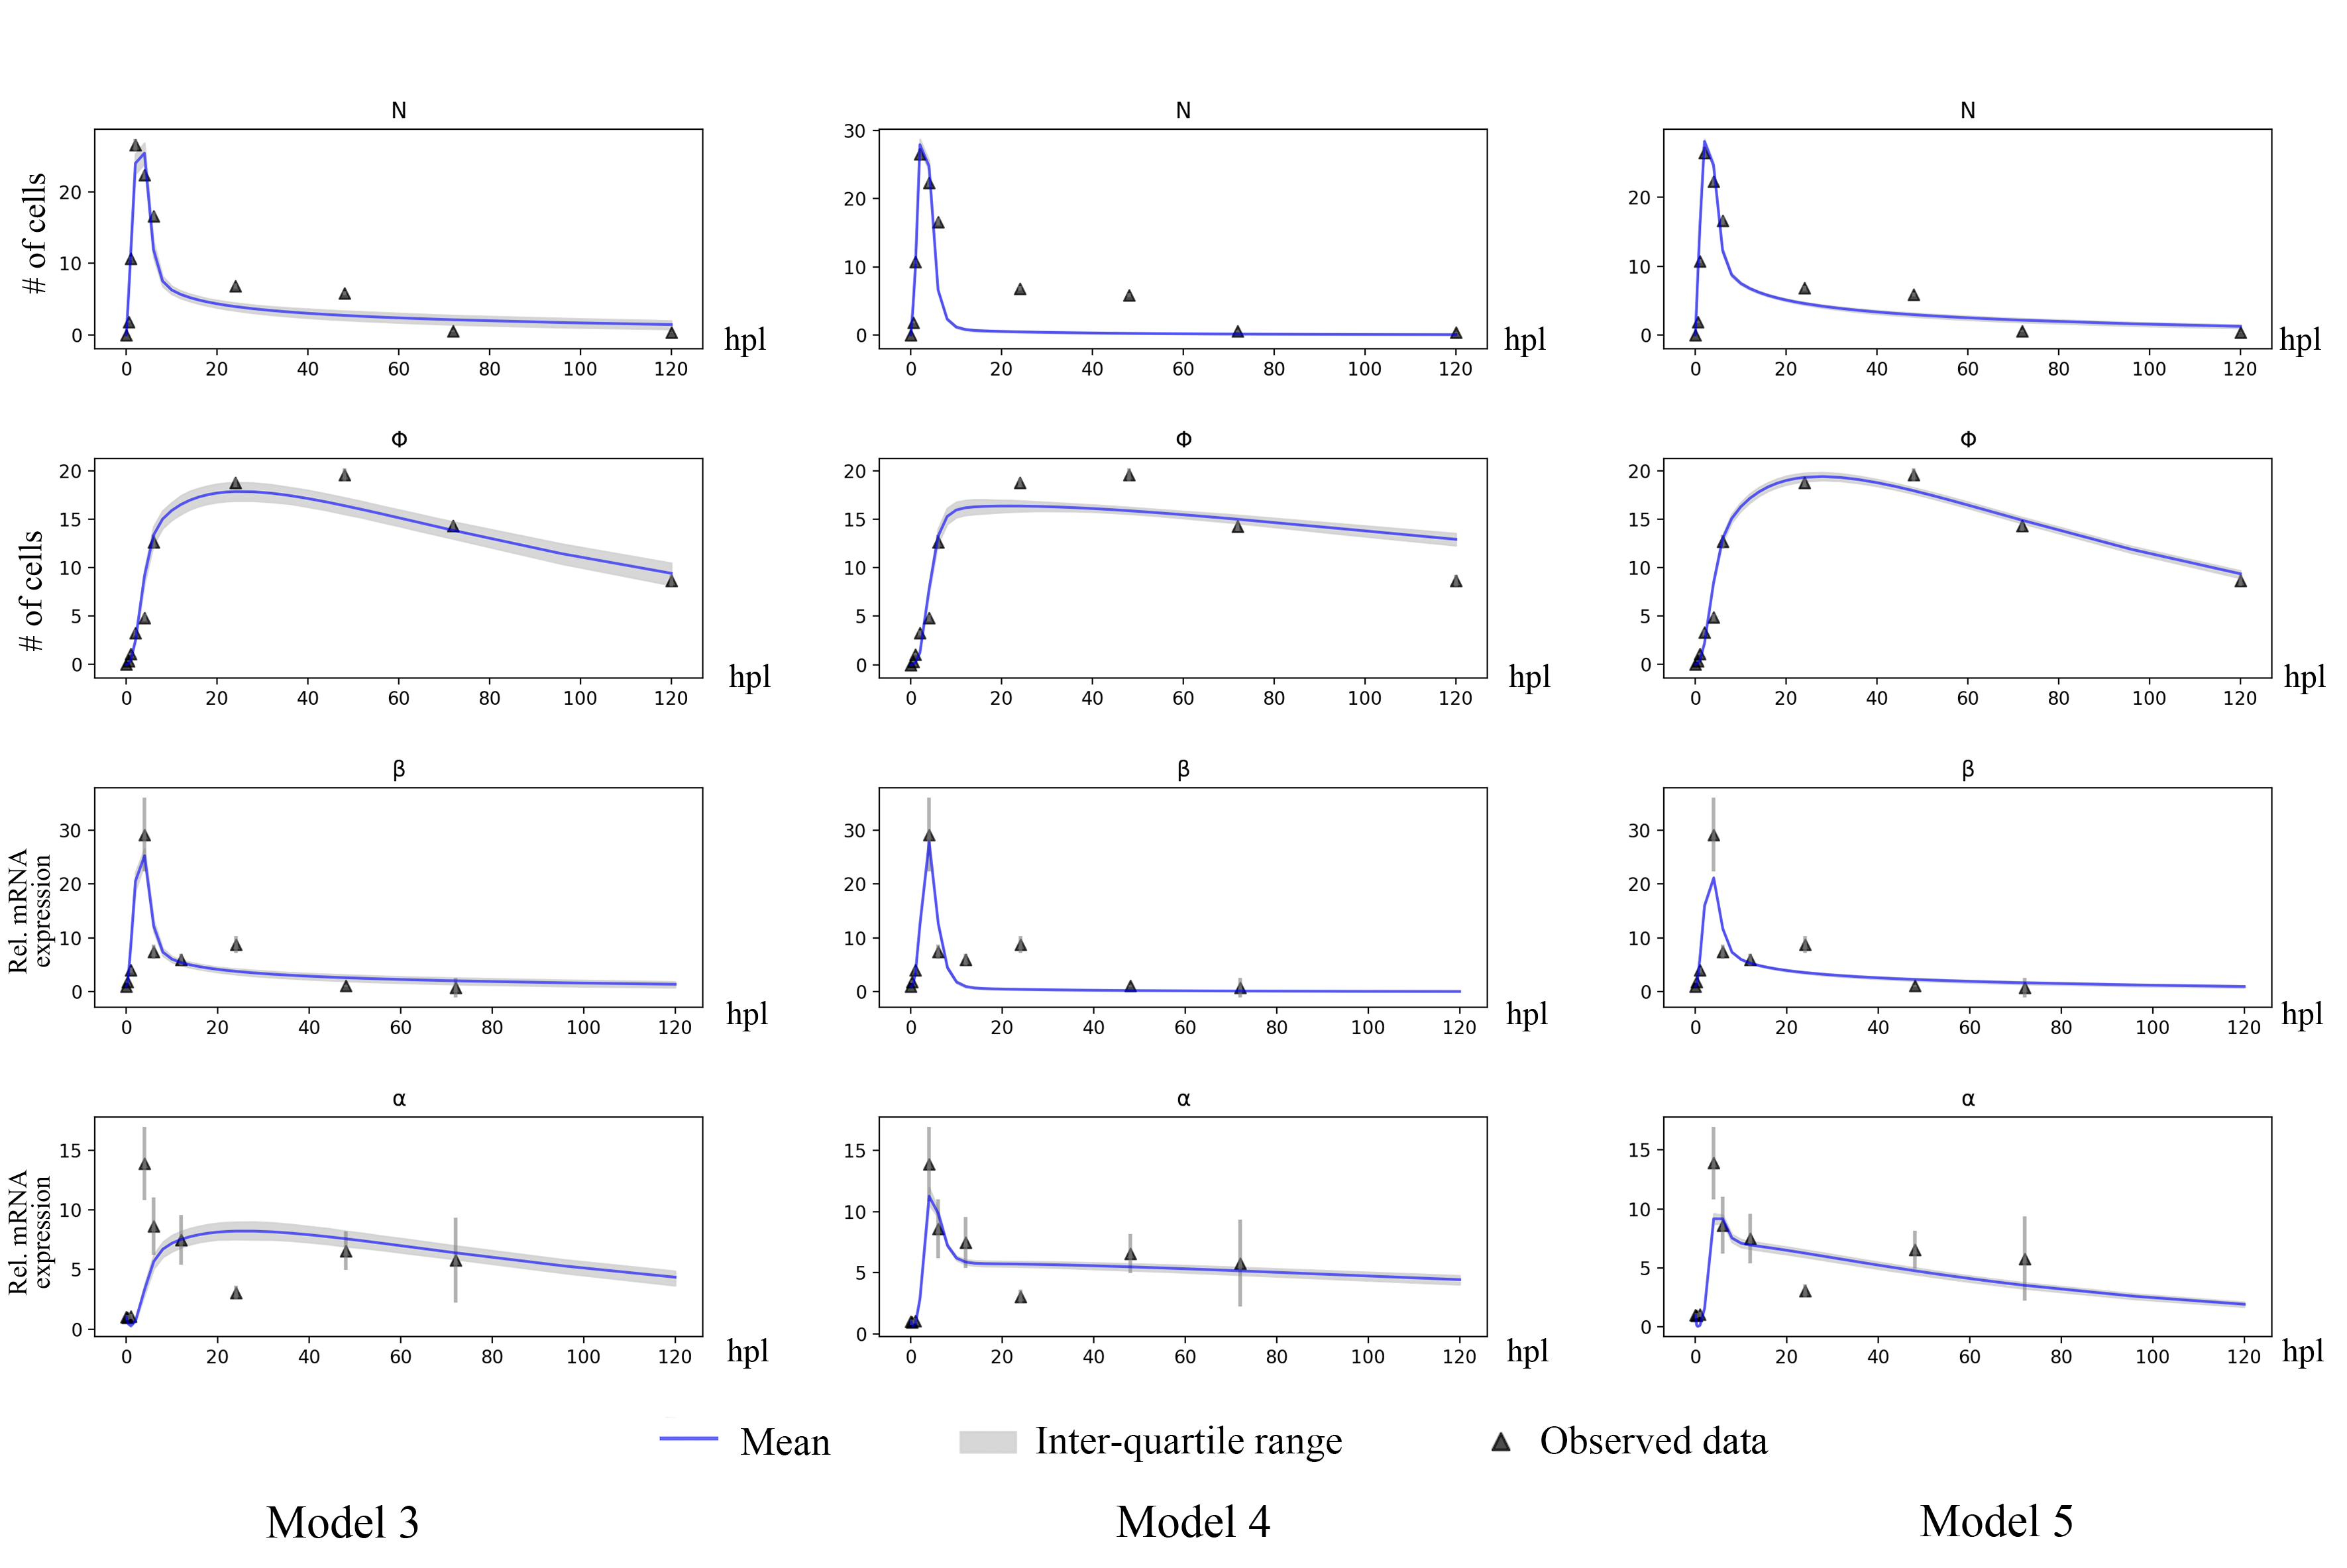
\includegraphics{fig/resultCurve345.png}}
    \end{center}

    \caption{Simulated data from the last population of model 3, 4 and 5}
    \label{fig:resultCurve345}

\end{figure}

\begin{figure}[ht]
    \begin{center}
        \resizebox{1.0\hsize}{!}{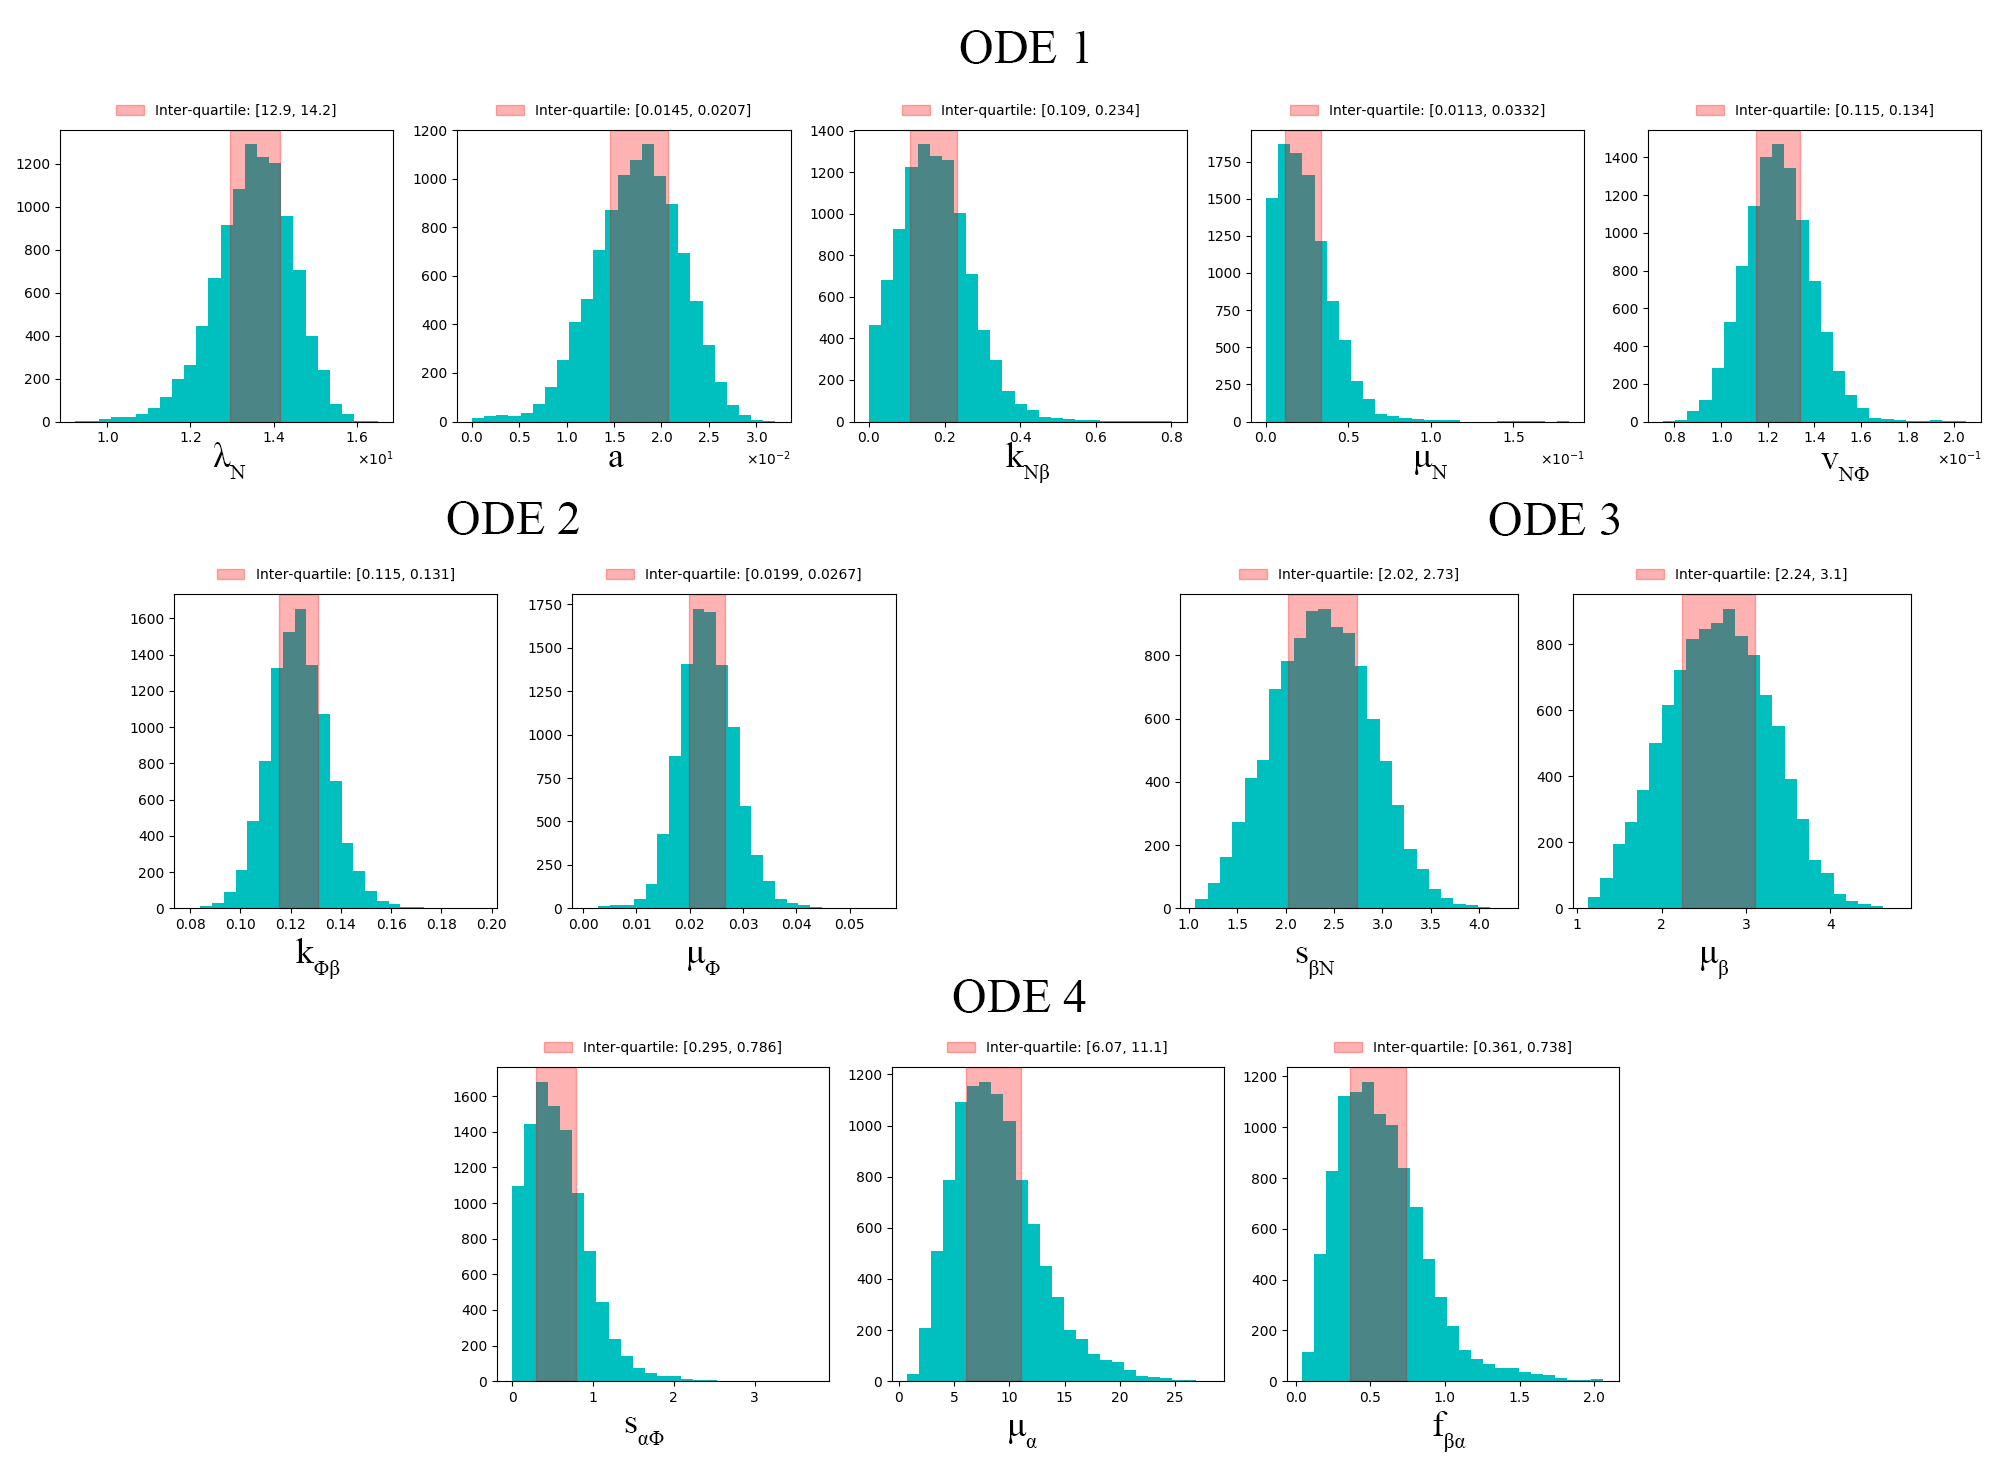
\includegraphics{fig/model5_para.png}}
    \end{center}

    \caption[Estimated posterior distribution of parameters in model 5]%
    {Estimated posterior distribution of parameters in model 5. Shaded range indicates 25\%--75\% quantile of the population}
    \label{fig:model5_para}

\end{figure}

By intuition model 4 and 5 would be the best models sofar that can recover most of observed data features. Model 1, 2 and 3 con also converge to a low final epsilon value (~20), but a key feature observed in target data -- a peak at around 4 hpl -- is not fitted. Some features, e.g. fluctuations in il-1$\beta$ and tnf-$alpha$ trajectories at around 20 hpl are still not ideally fitted; all existing models give a steady or gradually decrease trends for all the four variables after 20 hpl, and fluctuations in the observed data are fitted by smooth and steady curves.

\begin{table}[t!]
    \centering
    \begin{tabular}{|c c c|}
        \hline
        Parameter            & Mean value & Inter-quartile interval \\[0.5ex]
        \hline\hline
        $\lambda_N$          & 13.5       & [12.9, 14.2]            \\
        $a$                  & 0.0175     & [0.0145, 0.0207]        \\
        $\kappa_{N\beta}$    & 0.176      & [0.109, 0.234]          \\
        $\mu_N$              & 0.0239     & [0.0113, 0.0332]        \\
        $\nu_{N\Phi}$        & 0.125      & [0.115, 0.134]          \\
        \hline
        $\kappa_{\Phi\beta}$ & 0.123      & [0.115, 0.131]          \\
        $\mu_\Phi$           & 0.0234     & [0.0199, 0.0267]        \\
        \hline
        $s_{\beta N}$        & 2.38       & [2.02, 2.73]            \\
        $\mu_\beta$          & 2.67       & [2.24, 3.10]            \\
        \hline
        $s_{\alpha\Phi}$     & 0.574      & [0.295, 0.786]          \\
        $\mu_\alpha$         & 8.91       & [6.07, 11.1]            \\
        $f_{\beta\alpha}$    & 0.577      & [0.361, 0.738]          \\
        \hline
    \end{tabular}
    \caption[Inferred parameter values of model 5]
    {Inferred parameter values of model 5. MORE DETAIL(SUPER maxt-5)}
    \label{table:estimated5}
\end{table}

After applying factors, the results were not largely different. As expected, applying factors made the data points at first half (where exists most of the fluctuations) more `focused', however the inferred models are close to one without factors, which could indicate that for model 4 and 5, applying factors will not largely affect the final convergency and the resultant posterior.

When we are trying more populations, an `over-fitting' behaviour is observed at the trajectory of macrophage (FIGURE). In this case, the discrepancy of simulated data and observed data comes from the last 2 data point (72 hpl and 120 hpl).

\begin{figure}[h]
    \begin{center}
        \resizebox{1.0\hsize}{!}{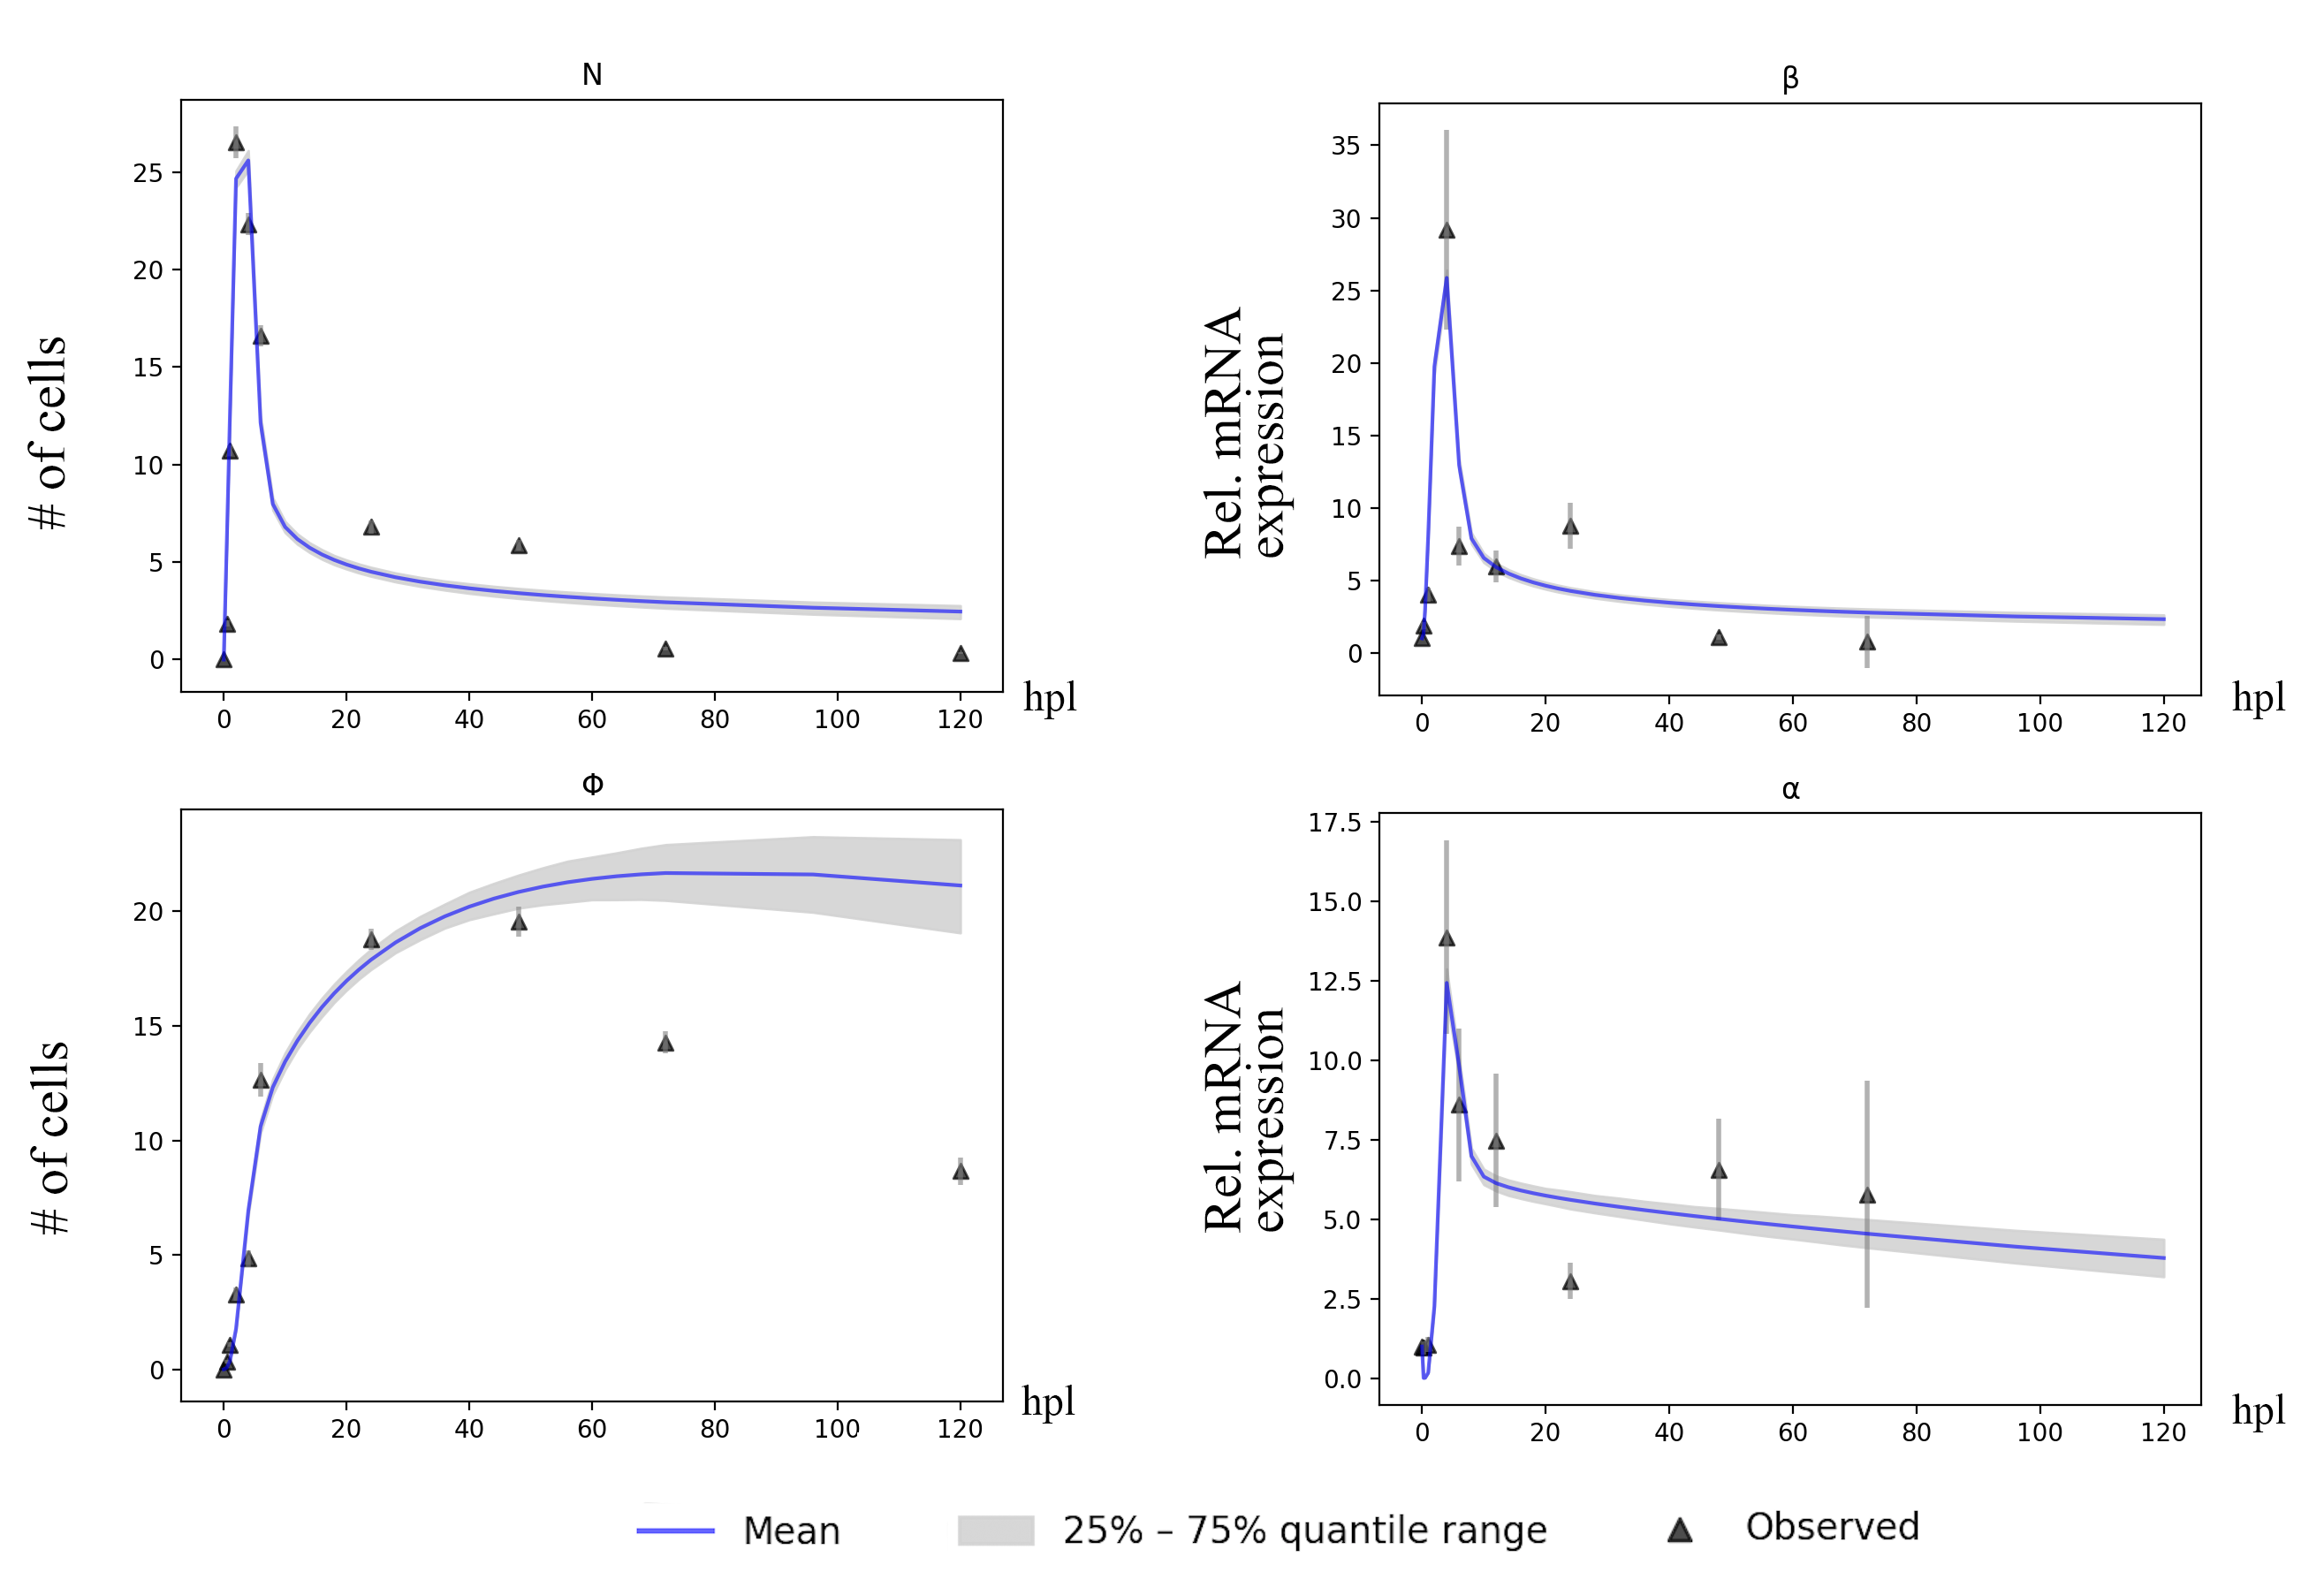
\includegraphics{fig/overfit.png}}
    \end{center}

    \caption[Simulated trajectory from the last population of model 5, with factors applied]{Simulated trajectory from the last population of model 5, with factors applied. MORE DETAIL}
    \label{fig:overfit}
\end{figure}

\begin{figure}[H]
    \begin{center}
        \resizebox{1.0\hsize}{!}{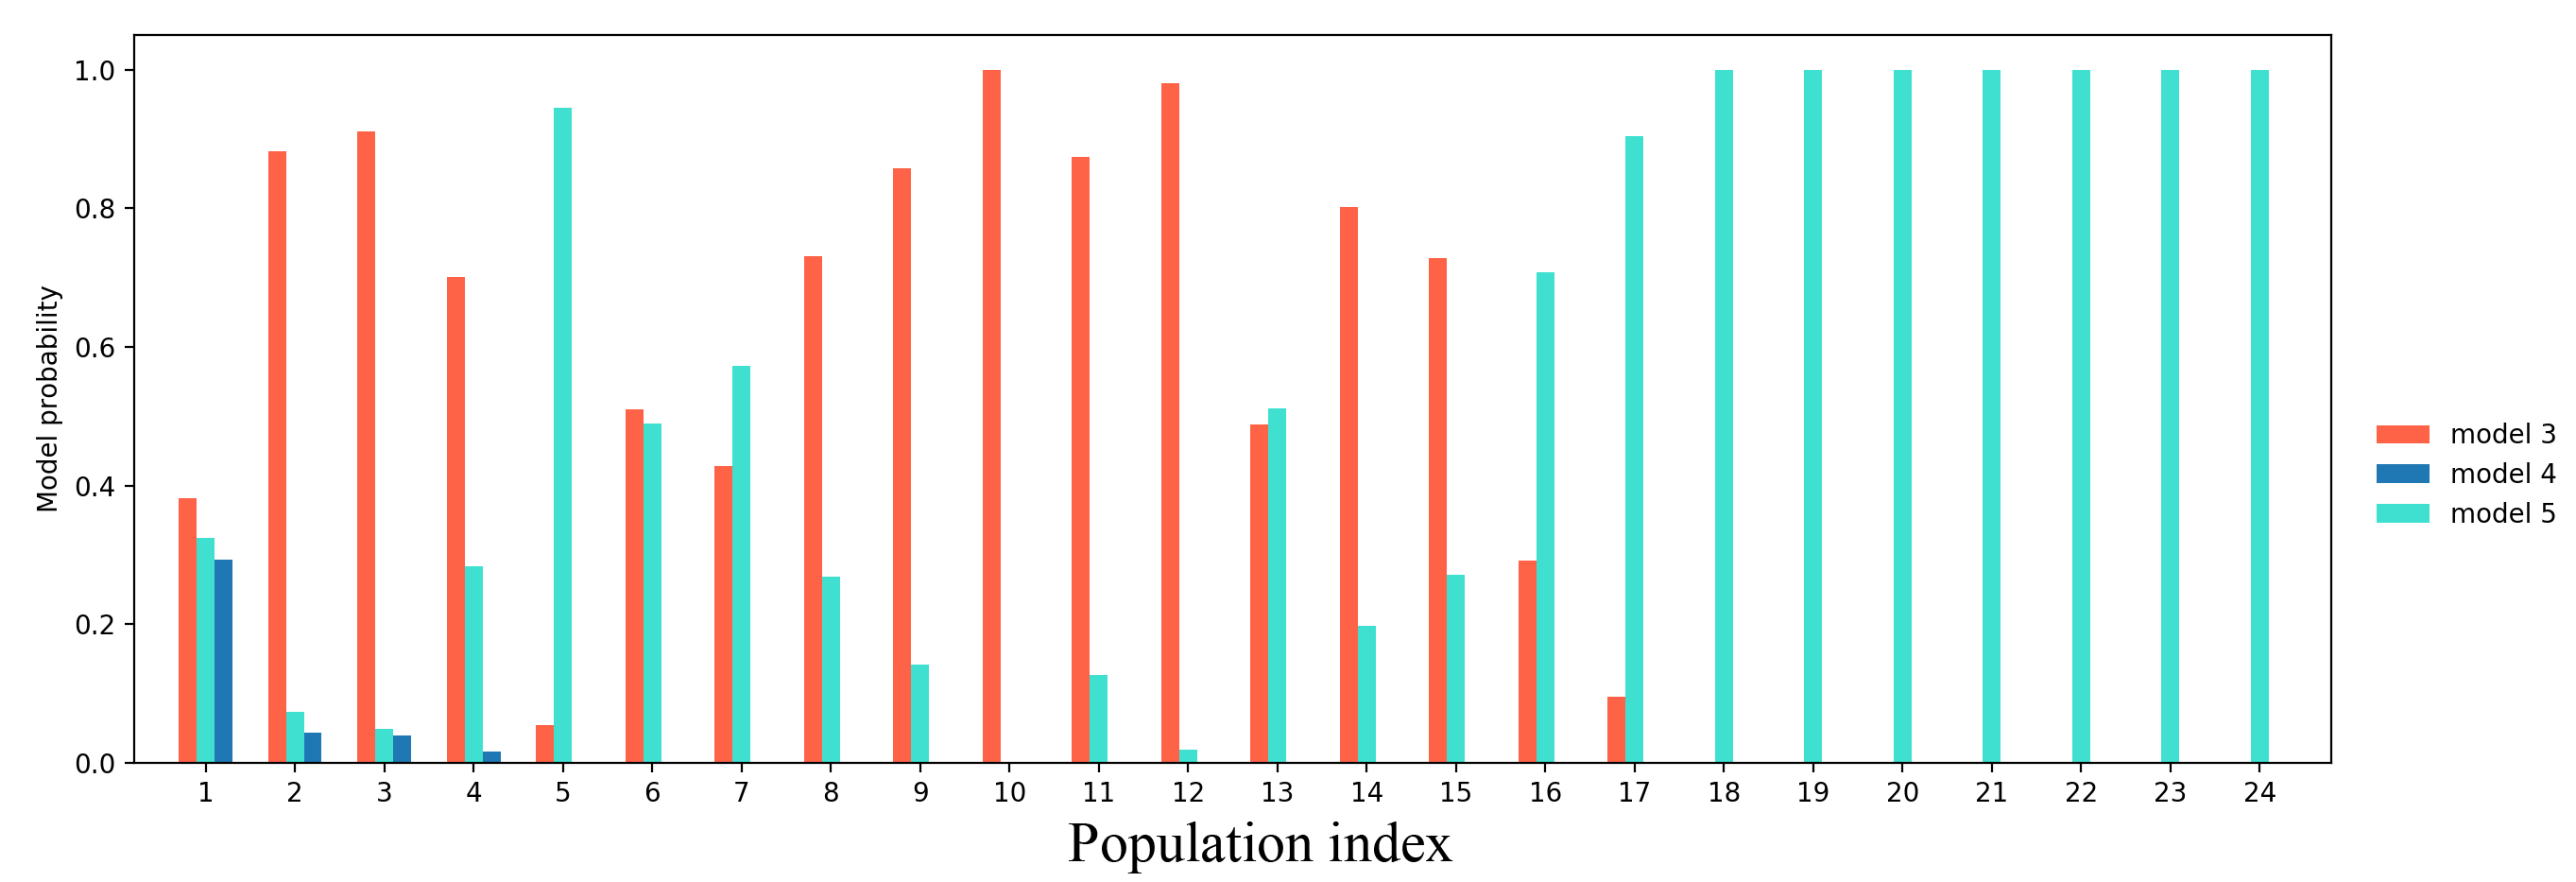
\includegraphics{fig/model345cmp.png}}
    \end{center}

    \caption[ABC SMC based model comparison of model 3, 4 and 5]{ABC SMC based model comparison of model 3, 4 and 5. MORE DETAIL}
    \label{fig:overfit}
\end{figure}


Next, we performed a model selection on model 3, 4 and 5. FIGURE shows the model probabilities at different generations. From population 10 to population 20 model 4 gains advantage but after population 20 model 5 is preferred. Again, as DISCUSSED in the model comparison of model 1, 2 and 3, we considered the the violently changing model probability is related to the inference ability at certain epsilon threshold values (epsilon) and possibly the insufficient exploration of the parameter space. Given the present result, model 5 is regarded as the best model. Some further experiments tried larger population size (10,000 particles per population) and more populations (36 populations), but the resultant model did not have a significantly better fit of the observed data, although much more computation resources are used.


A inferred parameter posterior distribution of model 5 is shown in FIGURE, the estimated mean values is shown in TABLE. SOME DESCRIPTION.


\subsection{Sensitivity of parameters}

[why last PCs]

[which parameters are most sensitive]

[compared to credible intervals plot]

[what does that mean]

A quick sensitivity analysis of the dynamical systems models can be quantified using principle component analysis (PCA) \cite{Toni}, where the first PCs corresponds to sloppy parameters while the last PCs corresponds to stiff parameters \cite{sensitivity}. PCA can only provide rough approximated sensitivity behaviour. As models 5 won in the model selection, a further interest is to explore the parameter-to-model sensitivity.

\begin{figure}[H]
    \begin{center}
        \resizebox{0.8\hsize}{!}{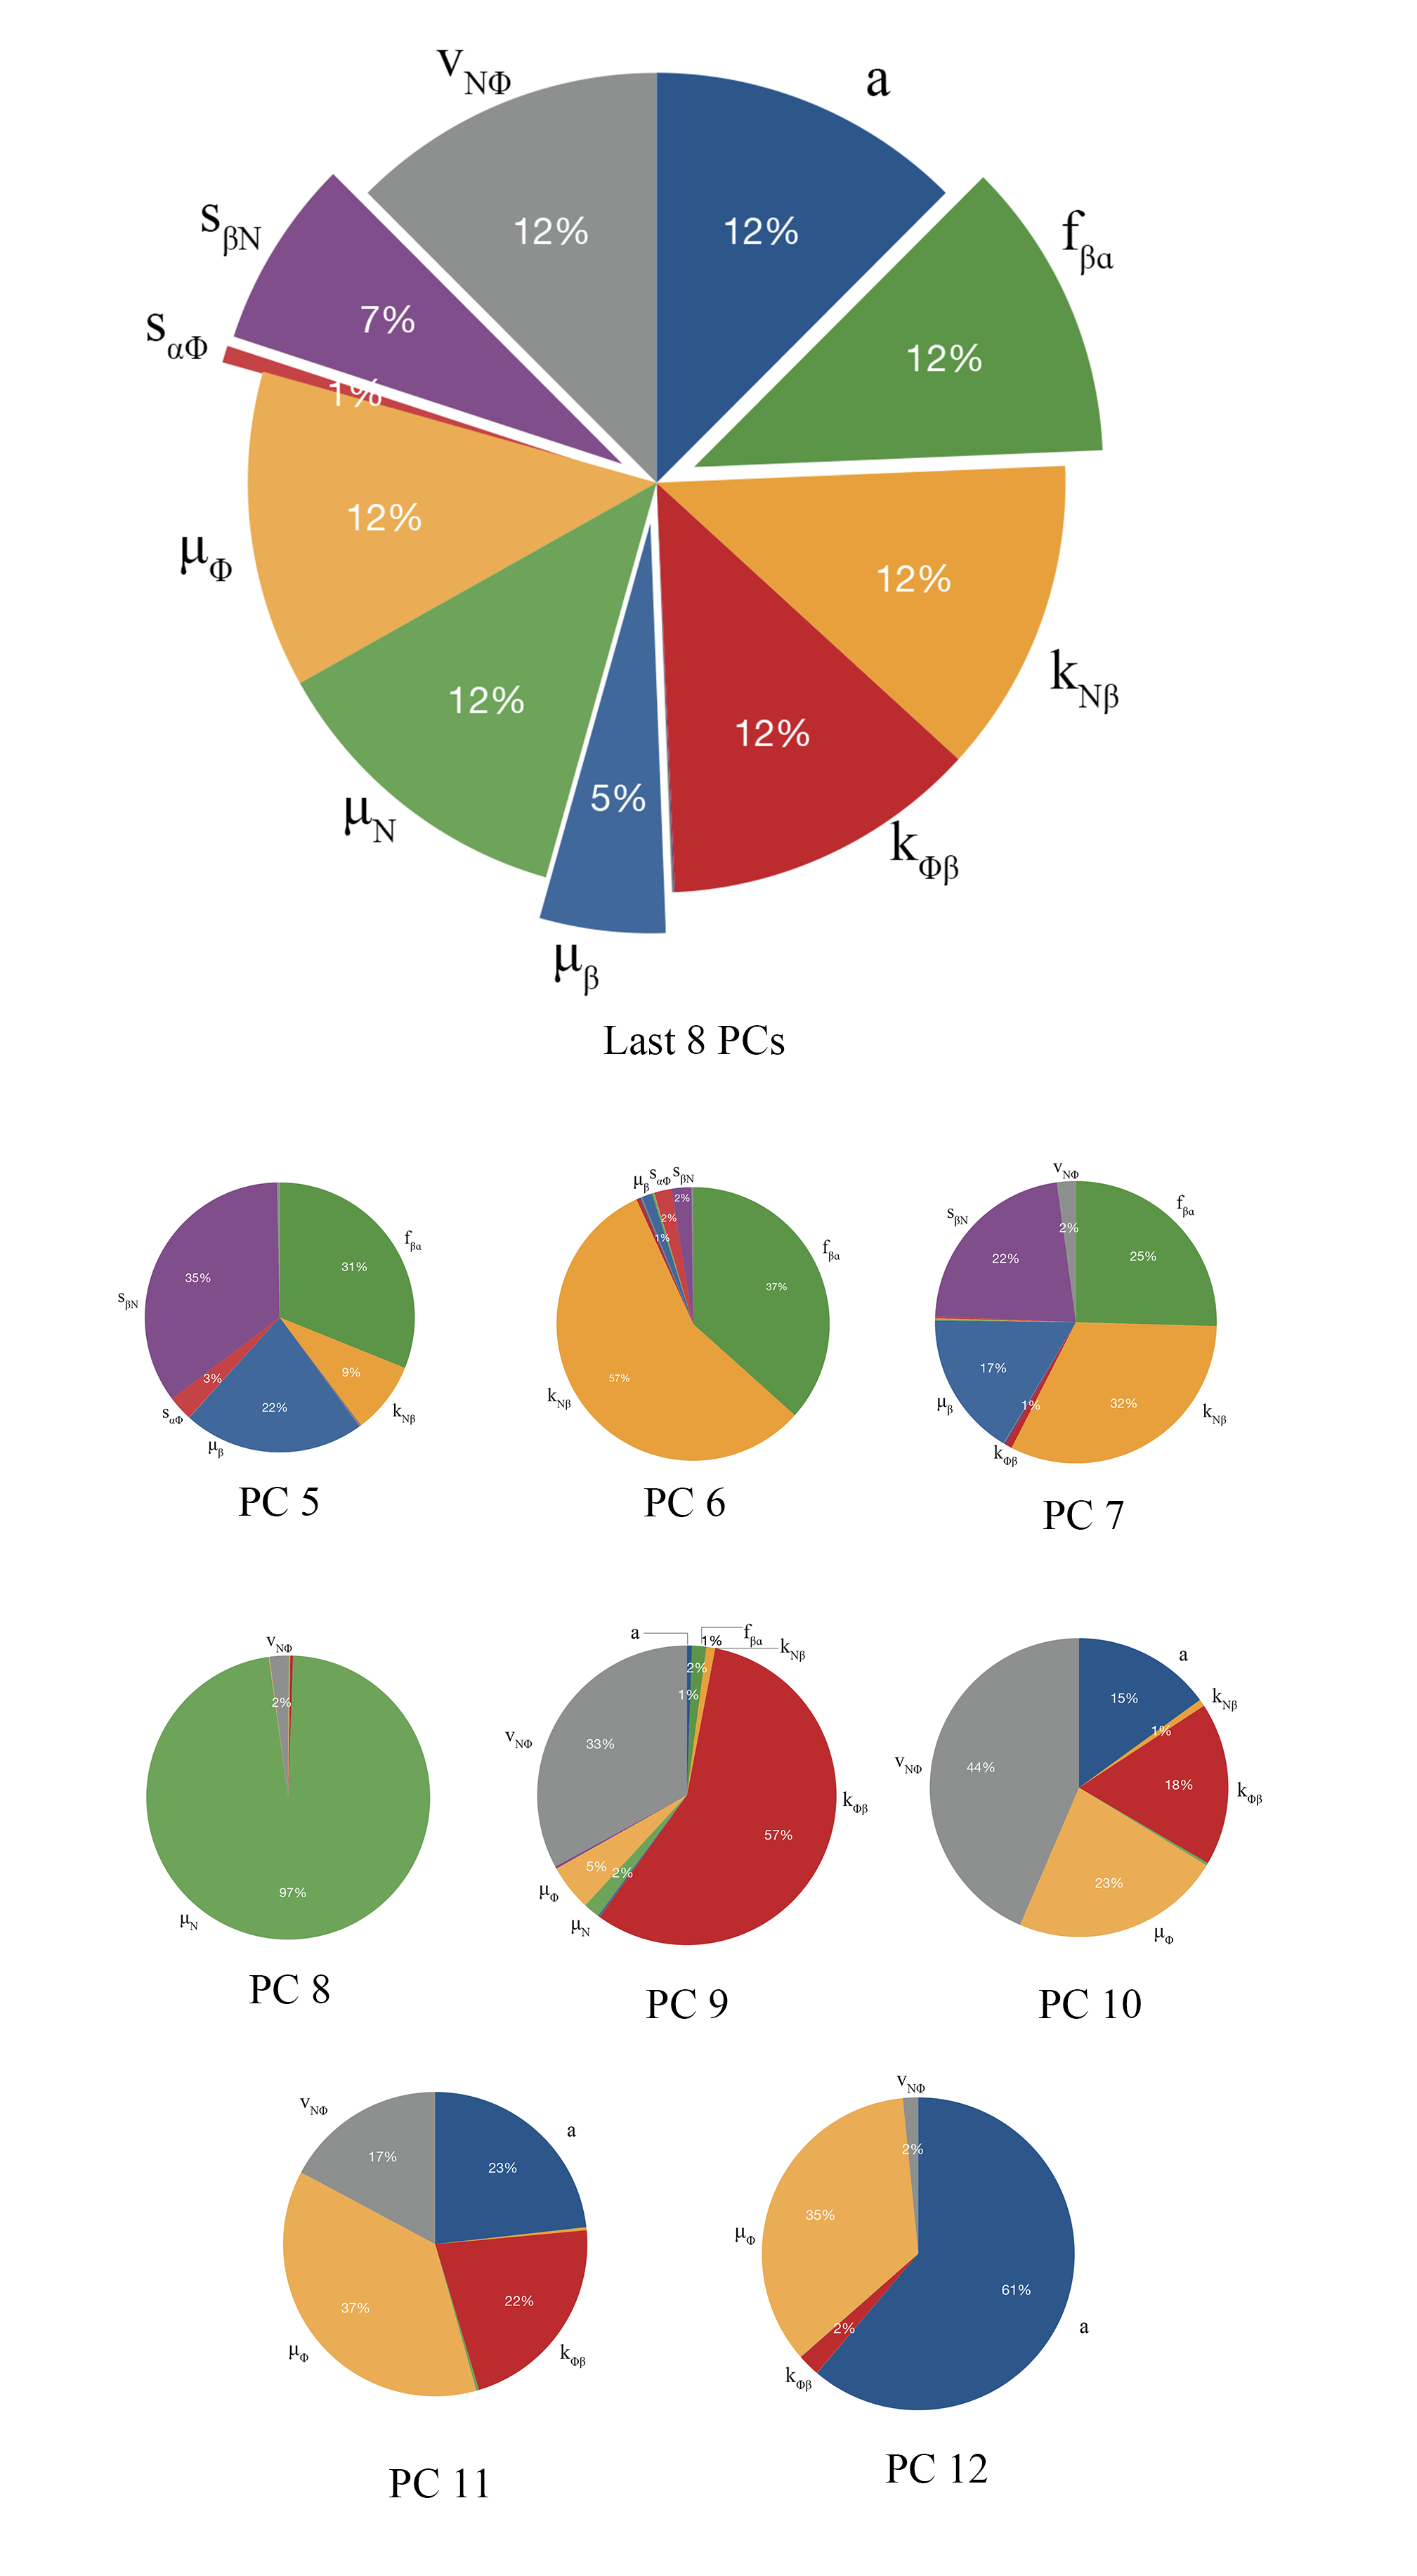
\includegraphics{fig/pc_pie_all.png}}
    \end{center}

    \caption[TODO]{PCA results of the last population of model 5. MORE DESCRIPTION}
    \label{fig:pc}
\end{figure}

\begin{figure}[H]
    \begin{center}
        \resizebox{1.0\hsize}{!}{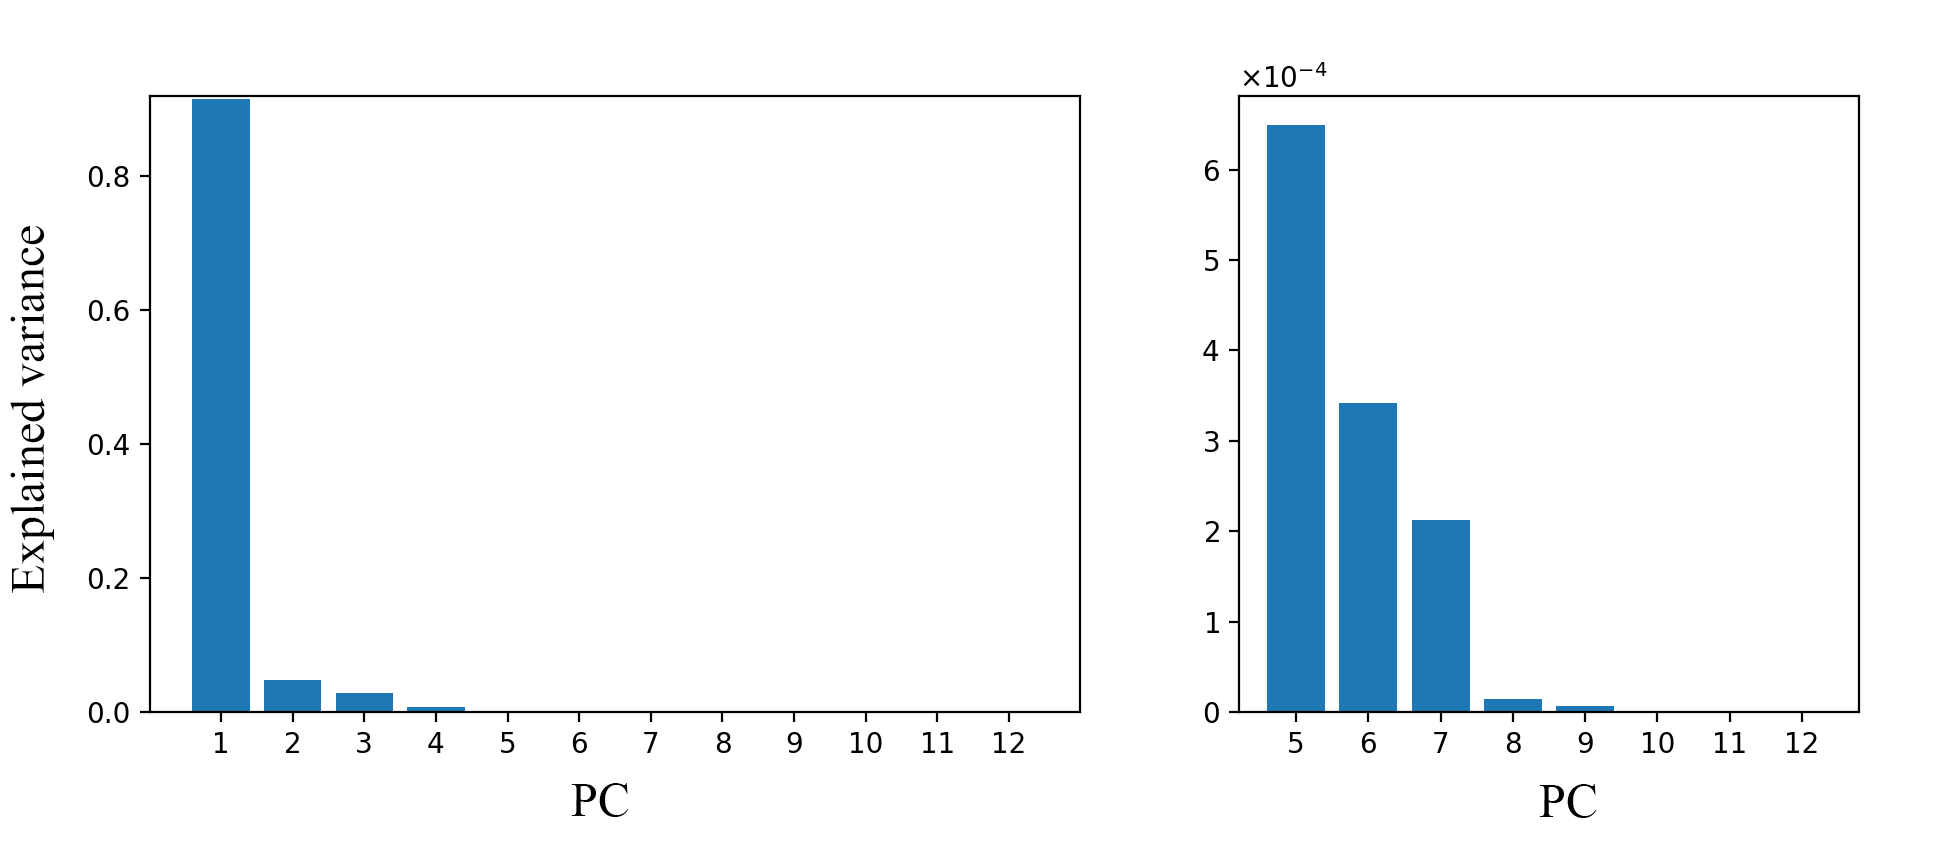
\includegraphics{fig/pc.png}}
    \end{center}

    \caption[PCA results of the last population of model 5]{PCA results of the last population of model 5. MORE DESCRIPTION}
    \label{fig:pc_pie}
\end{figure}


FIGURE shows the results of PCA on the last population of inferred model 5. The last PC (PC12) is mostly consists of the linear combination of $a$ (from the equation of neutrophil) and $\mu_\Phi$ (from the equation of macrophage), to which the model is most sensitive. If we conclude the last 5 PCs (FIGURE), then $v_{N\Phi}$, $\mu_N)$ (from the equation of neutrophil) and $k_{\Phi\beta}$ (from the equation of macrophage) contribute most portions together with $a$ and $\mu_\Phi$. As a conclusion, model 5 is sensitive to changes in the above parameters, which all come from the equation of neutrophil and macrophage i.e. equations of the cells; it may suggests that given the observed data, the inferred model is more sensitive to cells' dynamic rather than cytokines' dynamics.

Also, some visualisations of the last population agreed with conclusions from PCA. Approximated posteriors of the last population plotted in FIGURE and credible ranges of parameters across populations in FIGURE shows that the 5 parameters identified by PCA is indeed `stiff' parameters.
